\documentclass{article}

% NeurIPS 2026 style (default = main track, double-blind)
\usepackage{neurips_2026}

% Common packages
\usepackage[utf8]{inputenc}
\usepackage[T1]{fontenc}
\usepackage{hyperref}
\usepackage{url}
\usepackage{booktabs}
\usepackage{amsfonts}
\usepackage{nicefrac}
\usepackage{microtype}
\usepackage{xcolor}

% Colorblind-safe palette (Tol Bright)
\definecolor{TolBlue}{HTML}{4477AA}
\definecolor{TolCyan}{HTML}{66CCEE}
\definecolor{TolGreen}{HTML}{228833}
\definecolor{TolYellow}{HTML}{CCBB44}
\definecolor{TolRed}{HTML}{EE6677}
\definecolor{TolPurple}{HTML}{AA3377}
\definecolor{TolGrey}{HTML}{BBBBBB}

% Additional packages from the ICML version
\usepackage{graphicx}
\usepackage{subcaption}
\usepackage{wrapfig}
\usepackage{multirow}
\usepackage{tabularx}
\usepackage{threeparttable}
\usepackage{amsmath}
\usepackage{amssymb}
\usepackage{mathtools}
\usepackage{amsthm}
\usepackage{pifont}

% Plotting
\usepackage{tikz}
\usetikzlibrary{decorations.pathreplacing, arrows.meta}
\usepackage{pgfplots}
\pgfplotsset{compat=1.18}

% cleveref (load after hyperref)
\usepackage[capitalize,noabbrev]{cleveref}

%%%%%%%%%%%%%%%%%%%%%%%%%%%%%%%%
% THEOREMS
%%%%%%%%%%%%%%%%%%%%%%%%%%%%%%%%
\theoremstyle{plain}
\newtheorem{theorem}{Theorem}[section]
\newtheorem{proposition}[theorem]{Proposition}
\newtheorem{lemma}[theorem]{Lemma}
\newtheorem{corollary}[theorem]{Corollary}
\theoremstyle{definition}
\newtheorem{definition}[theorem]{Definition}
\newtheorem{assumption}[theorem]{Assumption}
\theoremstyle{remark}
\newtheorem{remark}[theorem]{Remark}

\title{LASER: A High-Fidelity Spike Representation SNN Framework \\ With Surrogate-Free Training}

\author{%
  Zhengzheng Tang \\
  Department of Computer Science\\
  Boston University\\
  Boston, MA, USA \\
  \texttt{zztangbu@bu.edu} \\
}

\begin{document}

\maketitle

\begin{abstract}
Spiking Neural Networks (SNNs) demonstrate great potential for energy-efficient computing due to their inherent event-driven sparsity, yet they face a long-standing challenge in matching the accuracy of Artificial Neural Networks (ANNs) due to errors from approximating continuous values with discrete spikes. To address this, we propose LASER, a high-fidelity spike representation SNN framework with surrogate-free training that introduces a precise bi-directional mapping for linear computation and a piecewise-approximate representation for nonlinear functions. Building on this high-fidelity forward propagation, we design an STE-based backpropagation strategy to ensure functional consistency with ANNs and enable stable training. Experiments validate that, unlike prior methods where errors diffuse across the network, LASER confines a slight error~(0.6\%) solely to the non-linear module. Consequently, LASER achieves over 50\% lower perplexity compared to state-of-the-art SNN frameworks with almost lossless accuracy.
\end{abstract}
\section{Introduction}
\label{sec:introduction}

% With the continuous expansion of parameter scales in large-scale multimodal ANNs such as language and vision models, the demand for computational resources and energy consumption is also increasing exponentially~\citep{tay2022efficient}. Although the transformer has become the standard, it still suffers from issues during the inference stage, such as redundant activations, low sparsity, high bandwidth usage, and high energy consumption~\citep{tay2022efficient}. These challenges have prompted researchers to reexamine more biologically inspired, sparsity-friendly neural network architectures~\citep{roy2019towards}. 


% Spiking Neural Networks (SNNs), known as the third generation of neural networks (Maass, 1996), are promising due to their low computational cost and biological plausibility. Inspired by biological neurons, SNNs utilize binary spikes for communication between neurons instead of numerical values. Compared to traditional Artificial Neural Networks (ANNs), SNNs achieve higher energy efficiency due to the parsity of event-driven signaling, particularly on neuromorphic hardware (Davies et al., 2018; DeBole et al., 2019; Peiet al., 2019).
% Among them, 
% Spiking Neural Networks (SNNs), with their event-driven, asynchronous computation and naturally sparse mechanisms, are considered an important direction for building highly energy-efficient neural network systems~\citep{roy2019towards}.
% Especially on neuromorphic chips such as Loihi, SNNs demonstrate better energy efficiency and lower latency compared to traditional ANNs~\citep{davies2018loihi,davies2021loihi}. 
% However, limited by their information expression capability, such as the complexity of information encoding and the difficulty of training, SNNs are still mainly applied to light image recognition or signal detection and are difficult to handle large-scale sequence modeling or natural language processing~\citep{roy2019towards,zheng2021going}.
% In recent years, exploratory works such as Spikeformer~\citep{} and SpikeGPT~\citep{} have attempted to scale SNNs to larger modeling scenarios and shown initial potential~\citep{zhou2023spikformer,zhu2023spikegpt,yao2023sdt}. 

% SNN 扩展到大模型有什么问题？
% tzz第一段背景：脉冲神经网络（Spiking Neural Networks, SNNs）作为第三代受生物神经系统启发的神经网络，因其事件驱动和高度稀疏的计算特性而受到广泛关注。与传统人工神经网络（Artificial Neural Networks, ANNs）依赖连续激活值进行全局同步计算不同，SNNs 通过离散脉冲在时间维度上传递信息，仅在事件发生时触发计算，从而在能效面展现出显著优势。尤其在类脑芯片等新型硬件上，SNNs 能够充分发挥稀疏与异步特性，为构建低功耗、可扩展的大规模智能系统提供了潜在路径。
% Spiking Neural Networks (SNNs), known as the third generation of neural networks inspired by biological neural systems~\citep{maass1997networks}, have attracted increasing attention due to their event-driven and highly sparse computational characteristics. Unlike traditional Artificial Neural Networks (ANNs), which rely on continuous activation values for synchronous and global computation~\citep{lecun2015deep}, SNNs transmit information through discrete spikes along the temporal dimension and trigger computation only when events occur. This unique mechanism leads to remarkable advantages in energy efficiency~\citep{roy2019towards}. Especially on neuromorphic chips such as Loihi, SNNs can fully exploit sparsity and asynchrony, demonstrating superior energy efficiency and lower latency compared to ANNs~\citep{davies2018loihi,davies2021loihi}, and providing a promising path toward low-power and scalable large-scale intelligent systems.

% 脉冲神经网络（Spiking Neural Networks, SNNs）因其事件驱动的稀疏性而被认为在能效与大规模智能系统中具有潜力~\citep{maass1997networks,roy2019towards,davies2018loihi,davies2021loihi}。
% SNNs在大规模建模场景中的核心问题是脉冲编码、非线性计算误差累积与梯度近似导致信息表达效率低、训练收敛慢且不稳定。Laser的核心思想是跳出现有对连续值近似的编码思维，提出一种全新的脉冲表达语言，实现离散脉冲序列和连续性的对应双向映射；对于非线性计算，引入可学习的结构化脉冲编码器，把非线性带来的近似误差作为可校准的残差吸纳到编码空间并重编码，其余网络保持线性算子与拓扑不变，实现高保真且结构一致的前向传播；在高保真且结构一致的前向传播基础上，我们可以使用STE使网络可训练而不需使用梯度近似。此时STE不再是“启发式替代项”，而是前向一致的等价映射，所以误差极小、收敛稳定。

% Spiking Neural Networks (SNNs) are promising for energy-efficient large-scale intelligence due to event-driven sparsity~\citep{maass1997networks,roy2019towards,davies2018loihi,davies2021loihi}. 

% 一句话解释一下现有SNN架构是怎么玩的
% Their main challenges lie in spike encoding, nonlinear error accumulation, and gradient approximation, 
% causing low representational efficiency and unstable training. Laser addresses these by introducing a spike expression language with exact bidirectional mapping between spikes and continuous values, and a learnable structured spike encoder that localizes nonlinear errors while keeping the rest of the network linear and topologically intact. With such high-fidelity forward consistency, the Straight-Through Estimator (STE) serves as an equivalent mapping rather than a heuristic, yielding minimal error and stable convergence.
% Spiking Neural Networks (SNNs) are considered promising for energy efficiency and large-scale intelligent systems due to their event-driven sparsity~\citep{maass1997networks,roy2019towards,davies2018loihi,davies2021loihi}.  
% In large-scale modeling, the core challenges of SNNs lie in spike encoding, error accumulation in nonlinear computation, and gradient approximation, which lead to low information representation efficiency, slow convergence, and unstable training.  
% The key idea of Laser is to break away from the conventional paradigm of approximating continuous values, and instead propose a new spike expression language that establishes a bidirectional mapping between discrete spike sequences and continuous values.  
% For nonlinear computation, a learnable structured spike encoder is introduced to absorb approximation errors from nonlinearities as calibratable residuals into the encoding space and re-encode them, while keeping the rest of the network linear and topologically unchanged, thereby achieving high-fidelity and structurally consistent forward propagation.  
% Based on this, the Straight-Through Estimator (STE) can be applied to make the network trainable without gradient approximation. In this setting, STE is no longer a “heuristic substitute” but a forward-consistent equivalent mapping, leading to minimal error and stable convergence.
% 上述问题并非只在某一个环节产生，而是会在编码、非线性和训练的每个环节都额外引入误差，并且这些误差会逐层累积。具体来说：(i) 线性编码方面，离散值近似连续纸本身本身就是近似过程，需要长时间积累才能逼近数值，因此在一开始就产生基础误差，并随网络传播扩散累积；(ii) 非线性处理方面，ReLU、Softmax等算子的脉冲实现缺乏高精度的近似方式，每一次非线性运算都会引入新的累积误差；(iii) 训练方面，离散脉冲的不可导性迫使现有方法依赖 surrogate gradient 或软替代，这些近似本身也会带来新的在网络中扩散误差。
% Spiking Neural Networks (SNNs) as the third generation of neural network models due to their unique neural dynamics and high biological plausibility, making them competitive candidates to Artificial Neural Networks (ANNs)~\citep{maass1997networks,roy2019towards,davies2018loihi,davies2021loihi}. 


\begin{wrapfigure}{r}{0.42\textwidth}
\vspace{-1em}
\centering
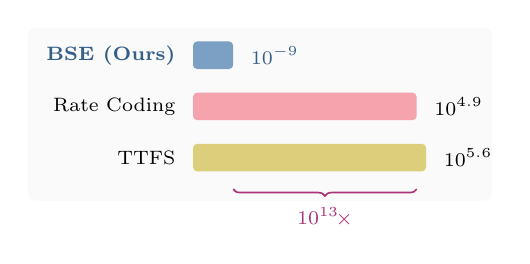
\begin{tikzpicture}[
    bar/.style={rounded corners=1.5pt, minimum height=0.35cm},
]
% Log scale mapping: log10(MSE) from -12 to 7, range=19, map to 3.2cm
% BSE:  (3/19)*3.2 = 0.51cm
% Rate: (16.89/19)*3.2 = 2.84cm
% TTFS: (17.57/19)*3.2 = 2.96cm

\def\yA{0}
\def\yB{-0.65}
\def\yC{-1.30}

% Background card
\fill[black!2, rounded corners=3pt] (-2.1, 0.35) rectangle (3.8, -1.85);

% Bars
\fill[TolBlue!70, bar] (0, \yA-0.175) rectangle (0.51, \yA+0.175);
\fill[TolRed!60, bar]  (0, \yB-0.175) rectangle (2.84, \yB+0.175);
\fill[TolYellow!70, bar] (0, \yC-0.175) rectangle (2.96, \yC+0.175);

% Method names (left)
\node[font=\scriptsize\bfseries, anchor=east, text=TolBlue!80!black] at (-0.1, \yA) {BSE (Ours)};
\node[font=\scriptsize, anchor=east] at (-0.1, \yB) {Rate Coding};
\node[font=\scriptsize, anchor=east] at (-0.1, \yC) {TTFS};

% Data values (right of bar)
\node[font=\scriptsize\bfseries, anchor=west, text=TolBlue!80!black] at (0.61, \yA) {$10^{-9}$};
\node[font=\scriptsize, anchor=west] at (2.94, \yB) {$10^{4.9}$};
\node[font=\scriptsize, anchor=west] at (3.06, \yC) {$10^{5.6}$};

% Gap brace
\draw[TolPurple, semithick, decorate, decoration={brace, amplitude=2.5pt, mirror}]
    (0.51, -1.7) -- (2.84, -1.7)
    node[midway, below=3pt, font=\scriptsize\bfseries, text=TolPurple] {$10^{13}\!\times$};

\end{tikzpicture}
\vspace{-0.3em}
\caption{Encoding MSE at $T\!=\!16$ steps (log scale). BSE achieves $10^{13}\!\times$ lower error than Rate Coding and TTFS.}
\label{fig:bse_fidelity}
\vspace{-1em}
\end{wrapfigure}
As the third generation of neural network models, Spiking Neural Networks (SNNs) distinguish themselves from Artificial Neural Networks (ANNs) by processing information via discrete spikes rather than continuous values, thereby closely emulating the firing dynamics of biological neurons. This event-driven mechanism grants SNNs a critical advantage in energy efficiency, positioning them as a compelling alternative for low-power applications and dedicated neuromorphic hardware \citep{maass1997networks,roy2019towards,davies2018loihi,davies2021loihi}.

However, the binary nature of spikes constrains the information representation capacity of SNN~\citep{auge2021encoding, guo2021coding}. This limitation compromises the achievement of both high-fidelity spike representation and the functionality required to match ANNs.
% spikes are binary events, so they not be able to represent as much information as continuous values used in ANNs~\citep{auge2021encoding,guo2021coding}.
% SNN faces issues of low representational efficiency and unstable training. This mainly arises from the inaccurate approximation of continuous activations by discrete spikes~\citep{auge2021encoding,guo2021coding}.
% \ding{172} During the encoding stage of converting ANNs into SNN spike representations, the use of discrete spikes to represent continuous values inherently introduces errors. To reduce this error, longer timesteps are required, leading to higher computational latency. As shown in Table~\ref{tab:bse_fidelity}, for the classic TTFS encoding~\citep{bonilla2022ttfs,stanojevic2024ttfs}, when the timestep is 1{,}024, the error is reduced by 14 orders of magnitude compared with 16, but the latency increases by 64 times. More critically, nonlinear computations lack a unified spike representation. Some works~\citep{zhou2023spikformer,yao2023sdt,spikedattention2024,wang2023stsa} propose replacing nonlinear operations with ``spike-friendly nonlinear structures''. But this method alters the network structure, undermining the carefully trained performance achieved within the original framework
\ding{172} During the encoding stage, converting continuous values into discrete spikes inevitably introduces approximation errors. 
% Reducing this error requires longer timesteps, which significantly increases computational latency. As shown in Table~\ref{tab:bse_fidelity}, in classical TTFS encoding~\citep{bonilla2022ttfs,stanojevic2024ttfs}, increasing the timestep from 16 to 1,024 reduces the error while increasing computation latency 64-fold.
Even worse, not all nonlinear function can be effectively represented by spikes (e.g., Softmax). 
% Some works propose replacing them with "spike-friendly" nonlinear structures~\citep{zhou2023spikformer,yao2023sdt,spikedattention2024,wang2023stsa}. This strategy alters the network architecture, undermining the carefully optimized performance achieved on the original network design.
% introducing additional training alignment costs.
\ding{173}In addition, enabling backpropagation for SNNs is essential for training but is complicated by the non-differentiable nature of spikes. 
% This forces researchers to use surrogate gradients or soft substitutes ~\citep{neftci2019surrogate,wu2018stbp,shrestha2018slayer,deng2022tet,zheng2021going}. 
% Such approximation methods introduce extra errors, making training unstable.
% This issue arises in three key aspects and the resulting errors accumulate layer by layer~\citep{rueckauer2017conversion,neftci2019surrogate}: 
% In addressing these issues, 
% existing methods often trade efficiency for low error: 
% To achieve the necessary model accuracy and functionality, 
% existing works typically rely on computation-intensive and surrogate solutions.

% mapping continuous values to discrete spikes is itself approximate and requires long timesteps to converge, thus introducing base errors from the start that accumulate during propagation (Table~\ref{tab:bse_fidelity})~\citep{rueckauer2017conversion,auge2021encoding,guo2021coding}; (ii) in nonlinear processing, spiking implementations of operators such as ReLU and Softmax lack precise approximations, so every nonlinear computation introduces new errors that further accumulate~\citep{rueckauer2017conversion,you2024spikeziptf,yao2023sdt,spikedattention2024}; (iii) in training, the non-differentiability of spikes forces the use of surrogate gradients or soft substitutes, which themselves introduce additional errors that diffuse through the network~\citep{neftci2019surrogate,wu2018stbp,shrestha2018slayer,deng2022tet,zheng2021going}.


% The fundamental problem of existing methods lies in the inaccurate approximation of continuous activations by discrete spikes~\citep{auge2021encoding,guo2021coding}. Such approximation is not confined to a single stage, but occurs in encoding, nonlinear processing, and training, where each stage introduces additional errors. These errors then accumulate layer by layer, forming error accumulation and diffusion, i.e., each layer generates its own error during computation, and the errors progressively accumulate and diffuse as they propagate forward and backward through the network~\citep{rueckauer2017conversion,neftci2019surrogate}. Specifically: (i) in terms of linear encoding, the mapping from continuous activations to discrete spikes is inherently approximate, requiring long timesteps to approach the target values. Thus, base errors are introduced from the very beginning and then accumulate and diffuse as they propagate through the network (Table~\ref{tab:bse_fidelity})~\citep{rueckauer2017conversion,auge2021encoding,guo2021coding}; (ii) in terms of nonlinear processing, spiking implementations of operators such as ReLU and Softmax lack high-precision approximations, so each nonlinear operation introduces new errors that further accumulate and diffuse~\citep{rueckauer2017conversion,you2024spikeziptf,yao2023sdt,spikedattention2024}; (iii) in terms of training, the non-differentiability of discrete spikes forces existing methods to rely on surrogate gradients or soft substitutes, and these approximations themselves introduce new errors that accumulate and diffuse through the network~\citep{neftci2019surrogate,wu2018stbp,shrestha2018slayer,deng2022tet,zheng2021going}.


% The fundamental problem of existing methods lies in the inaccurate approximation of continuous activations by discrete spikes~\citep{auge2021encoding,guo2021coding}. Such approximation does not occur in a single stage only, but introduces additional errors in encoding, nonlinear processing, and training, and these errors accumulate and diffuse progressively with network depth~\citep{rueckauer2017conversion,neftci2019surrogate}, 

% % as illustrated in Figure~\ref{fig:error_diffusion_localization}.
% Specifically: (i) in terms of linear encoding, the approximation of discrete values to continuous activations is itself an approximation process, requiring long timesteps to approach numerical values, thereby introducing base errors from the very beginning and accumulating as they propagate through the network (see Table~\ref{tab:bse_fidelity})~\citep{rueckauer2017conversion,auge2021encoding,guo2021coding}; (ii) in terms of nonlinear processing, spiking implementations of operators such as ReLU and Softmax lack high-precision approximation methods, so each nonlinear operation introduces new cumulative errors~\citep{rueckauer2017conversion,you2024spikeziptf,yao2023sdt,spikedattention2024}; (iii) in terms of training, the non-differentiability of discrete spikes forces existing methods to rely on surrogate gradients or soft substitutes, which themselves introduce new errors that further diffuse through the network~\citep{neftci2019surrogate,wu2018stbp,shrestha2018slayer,deng2022tet,zheng2021going}.

% \begin{figure}[t]
%     \centering
%     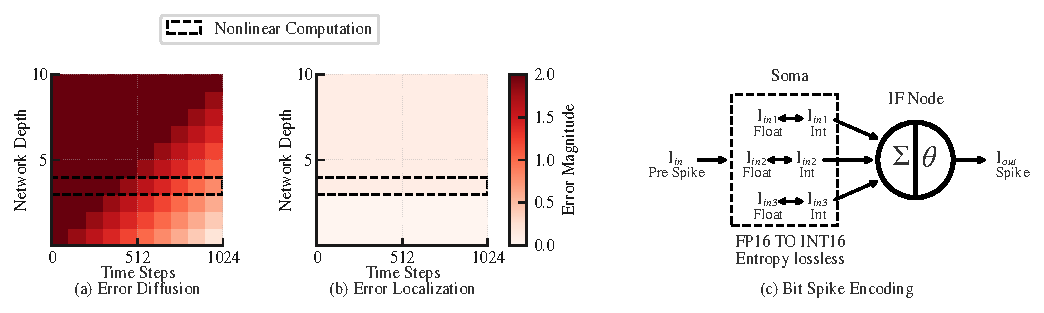
\includegraphics[width=0.85\linewidth]{figures/error_diffusion.pdf}
%     \caption{Comparison of error accumulation–diffusion and error localization: (a) Conventional methods introduce errors at multiple stages, which progressively accumulate and diffuse with network depth and timesteps; (b) In LASER, linear computations remain lossless, and errors are strictly confined to a single nonlinear module without layer-wise accumulation or diffusion; (c) Bit Spike Encoding (BSE) maps an $N$-bit integer to its corresponding $N$-bit binary spike sequence to achieve exact losslessness, and for floating-point representations it also preserves the same information entropy and machine precision as the original values (see Appendix~\ref{app:bse_entropy_proof}).
% }
%     \label{fig:error_diffusion_localization}
% \end{figure}

% \begin{table}[t]
% \centering
% \caption{Reconstruction fidelity (MSE; mean $\pm$ std over 10{,}000 random values) with explicit precision and latency cost (Time Steps). BSE attains $10^{11}$–$10^{18}$ lower error than rate coding and TTFS under the same step budgets, reaching near-machine precision at FP32. Notably, TTFS requires as many as 1{,}024 time steps to match the fidelity that BSE already achieves within 16 steps, highlighting the substantially higher latency cost of TTFS.}
% \label{tab:bse_fidelity}
% \begin{tabular}{lccc}
% \hline
% \textbf{Encoding Scheme} & \textbf{Time Steps} & \textbf{MSE (mean $\pm$ std)} \\
% \hline
% Rate Coding     & 16   & $7.70\pm 0.02 \times 10^{4}$ \\
% Rate Coding     & 32   & $4.46\pm 0.01 \times 10^{4}$ \\
% TTFS      & 16   & $3.68\pm 0.02 \times 10^{5}$ \\
% TTFS      & 32   & $6.03\pm 0.01 \times 10^{4}$ \\
% TTFS      & 1024 & $1.03\pm 0.01 \times 10^{-9}$ \\
% \textbf{Ours}& 2    & $\mathbf{9.26\pm 0.04 \times 10^{4}}$ \\
% \textbf{Ours}& 4    & $\mathbf{3.70\pm 0.03 \times 10^{-4}}$ \\
% \textbf{Ours}& 8    & $\mathbf{1.28\pm 0.01 \times 10^{-6}}$ \\
% \textbf{Ours}& 16   & $\mathbf{1.03\pm 0.02 \times 10^{-9}}$ \\
% \textbf{Ours}& 32   & $\mathbf{1.33\pm 0.01 \times 10^{-14}}$ \\
% \hline
% \end{tabular}
% \end{table}
% [Data Source] Original table kept for reference during revision
% \begin{table}[t]
% \centering
% \caption{Reconstruction fidelity (MSE; mean $\pm$ std over 10{,}000 random values) with explicit precision and latency cost (Time Steps). BSE attains $10^{11}$–$10^{18}$ lower error than rate coding and TTFS under the same step budgets, reaching near-machine precision at FP32. Notably, TTFS requires as many as 1{,}024 time steps to match the fidelity that BSE already achieves within 16 steps, highlighting the substantially higher latency cost of TTFS.}
% \label{tab:bse_fidelity}
% \resizebox{\textwidth}{!}{%
% \begin{tabular}{lcc}
% \hline
% \textbf{Encoding Scheme} & \textbf{Time Steps} & \textbf{MSE (mean $\pm$ std)} \\
% \hline
% Rate Coding      & 16   & $7.70\pm 0.02 \times 10^{4}$ \\
% Rate Coding      & 32   & $4.46\pm 0.01 \times 10^{4}$ \\
% TTFS             & 16   & $3.68\pm 0.02 \times 10^{5}$ \\
% TTFS             & 32   & $6.03\pm 0.01 \times 10^{4}$ \\
% TTFS             & 1024 & $1.03\pm 0.01 \times 10^{-9}$ \\
% \textbf{Ours}    & 2    & $\mathbf{9.26\pm 0.04 \times 10^{4}}$ \\
% \textbf{Ours}    & 4    & $\mathbf{3.70\pm 0.03 \times 10^{-4}}$ \\
% \textbf{Ours}    & 8    & $\mathbf{1.28\pm 0.01 \times 10^{-6}}$ \\
% \textbf{Ours}    & 16   & $\mathbf{1.03\pm 0.02 \times 10^{-9}}$ \\
% \textbf{Ours}    & 32   & $\mathbf{1.33\pm 0.01 \times 10^{-14}}$ \\
% \hline
% \end{tabular}%
% }
% \end{table}

% [Data Source] Figure 1 original table data
% Rate Coding: T=16 → 7.70e4, T=32 → 4.46e4
% TTFS: T=16 → 3.68e5, T=32 → 6.03e4, T=1024 → 1.03e-9
% BSE: T=2 → 9.26e4, T=4 → 3.70e-4, T=8 → 1.28e-6, T=16 → 1.03e-9, T=32 → 1.33e-14

To achieve the high-fidelity spike representation and functionality, existing works typically rely on computation-intensive and surrogate solutions, which come at the cost of either efficiency or accuracy.
% In addressing these issues, existing works typically rely on computation-intensive and surrogate solutions. 
% 这是以牺牲效率或准确率为代价的
First, existing works rely on additional computation to compensate for errors introduced during the encoding process. Specifically,
% First, to enhance the precision of spike encoding, 
longer timesteps are often employed, which significantly increases computational latency. As shown in Figure~\ref{fig:bse_fidelity}, in classical TTFS encoding~\citep{bonilla2022ttfs,stanojevic2024ttfs}, increasing the timestep from 16 to 1,024 reduces the error while increasing computation latency 64-fold.
Second, these works use surrogate techniques to enable spike representation of nonlinear functions.
% spike-based computation of nonlinear functions and support backpropagation~\citep{zhou2023spikformer, yao2023sdt, spikedattention2024, wang2023stsa,neftci2019surrogate, wu2018stbp, shrestha2018slayer, deng2022tet, zheng2021going}. 
For example, they replace activation functions with ``spike-friendly'' ReLU
% they replace nonlinear functions with "spike-friendly" structures to implement spike representation of these nonlinear functions
~\citep{zhou2023spikformer, yao2023sdt, spikedattention2024}. This strategy alters the network architecture, undermining the carefully optimized performance achieved on the original network design.
Finally, these works using surrogate gradients or soft substitutes to achieve backpropagation based on spike representation~\citep{neftci2019surrogate, shrestha2018slayer, deng2022tet}. Such approximation methods introduce extra errors, making training unstable.
% 这里怎么引入误差扩散？
% Second, to achieve spike representation of nonlinear functions, 
% For example, replacing nonlinear functions with "spike-friendly" structures \citep{zhou2023spikformer, yao2023sdt, spikedattention2024, wang2023stsa}. 
% Consequently, additional training alignment costs are required to restore performance.
% use surrogate gradients/soft substitutes to support training of networks based on spike representations, researchers are forced to use surrogate gradients or soft substitutes \citep{neftci2019surrogate, wu2018stbp, shrestha2018slayer, deng2022tet, zheng2021going}. 
% However, these approximation strategies change the network's architecture or introduce extra errors, ultimately compromising model's final performance and stability.
% Second, 为实现非线性函数的脉冲表达，some works propose replacing them with "spike-friendly" nonlinear structures~\citep{zhou2023spikformer,yao2023sdt,spikedattention2024,wang2023stsa}. This strategy alters the network architecture, undermining the carefully optimized performance achieved on the original network design. 需要额外的训练来对齐性能。
% % introducing additional training alignment costs.

% 最后，为支持基于脉冲表示的网络训练，This forces researchers to use surrogate gradients or soft substitutes ~\citep{neftci2019surrogate,wu2018stbp,shrestha2018slayer,deng2022tet,zheng2021going}. 
% Such approximation methods introduce extra errors, making training unstable.

% (i) For linear encoding, they rely on long time windows to improve approximation precision, but this significantly increases latency and energy consumption, reducing inference efficiency~\citep{guo2021coding,bu2023ultralow,you2024spikeziptf}; (ii) in nonlinear processing, they adopt structural rewrites or spike-friendly substitutes (e.g., replacing activation functions with ReLU) to maintain model functionality and expressiveness, but these introduce extra computation and training alignment overhead, essentially sacrificing efficiency as well~\citep{zhou2023spikformer,zhou2024spikformerv2,yao2023sdt,spikedattention2024,tang2024sorbet,you2024spikeziptf}; (iii) in the training stage, methods such as BackPropagation Through Time (BPTT) combined with surrogate gradients improve training stability. However, BPTT must store the states of all timesteps, causing latency and memory overhead to grow rapidly with network scale~\citep{wu2018stbp,shrestha2018slayer,neftci2019surrogate,deng2022tet,zheng2021going}.


% 因此，我们提出 LASER，一个误差有界的脉冲表示框架。该框架不做全局近似（下个定义，和前面反复提的误差累积对应起来），先以一种低延迟的精确双向映射编码方式，保证了离散脉冲与ANN连续激活值的一致性，同时使用分段自适应策略拟合非线性曲线，同时保持输出均为脉冲编码格式，从而不做结构上的牺牲完成脉冲空间里的端到端推理，误差固定在单一的非线性位置，使前向路径保持与ANN的等价。正是由于我们的高保真前向传播，可以使用STE替代导数而不改变数值路径，做到收敛稳定，误差不随时间与深度扩散。
% In this paper, Instead of applying global approximations, we propose LASER, an error-bounded spiking representation framework, 且不损失效率. 主要贡献如下：
% \begin{itemize}

% 现在的：
    % \item 我们首次提出离散脉冲与连续值的精确对应编码方式 Bit Spike Encoding (BSE)。其核心思想是通过同位宽量化将浮点数转化为整数，保持与原始数值相同的信息熵和机器精度（证明见附录~\ref{app:bse_entropy_proof}），并利用固定的短时间窗，将整数数值映射为与其二进制表示一致的脉冲序列。
    % \item 在 BSE 编码的基础上我们提出自适应脉冲编解码器（ASNC），用于非线性计算，与现有方法需要进行大规模结构替换不同，ASNC 作为结构化逼近器无需改写网络结构，即可在脉冲域完成任意非线性的局部近似，保持整体结构路径一致，无需训练对齐。
    % \item 在高保真的前向传播基础上，我们引入恒等梯度代理（STE）替代导数，实现了稳定收敛的脉冲神经网络训练。由于我们的前向传播没有对网络进行结构上的改变，因此梯度路径与数值路径完全对齐，反向传播不会额外改变计算过程，从而保证了训练的收敛稳定。



    %     \item 我们首先提出无损确定性脉冲编码 Bit Spike Encoding，而不是在既有压缩方案上做降低损失。BSE 的核心思想是利用固定的短时间窗，将一个数值拆解为稀疏有序的脉冲序列，每个时间步对应一位二进制比特。这样 $N$ 个时间步可以完整表示 Int$N$ 的所有数值范围，同时通过同位宽量化在浮点数表示上保持与原始数值相同的信息熵和机器精度（证明见附录~\ref{app:bse_entropy_proof}）。在这种编码下，数值的编码和解码互为确定过程，所有线性计算都可以直接在脉冲域执行，得到的结果与在原始数值域中的计算完全一致，因此不会引入额外误差。与之形成对比的是，传统的编码方式依赖长时间窗来提高近似精度，本身存在不可逆近似损失，导致误差会随着深度累积扩散。BSE 通过确定性和可逆性消除了线性计算这一扩散路径，为后续将误差固定在非线性近似模块、实现稳定训练和大规模扩展奠定基础。
    % \item 我们首先提出无损且确定性的脉冲编码 Bit Spike Encoding (BSE)，而非仅在既有压缩方案上减少损失。其核心思想是通过同位宽量化将浮点数转化为整数，保持与原始数值相同的信息熵和机器精度（证明见附录~\ref{app:bse_entropy_proof}），并利用固定的短时间窗，将 Int$N$ 数值映射为与其二进制表示一致的 $N$ 个时间步脉冲序列。在这种编码下，编码与解码互为确定过程，所有线性计算可直接在脉冲域执行且结果与数值域完全一致，从而消除线性计算中的误差扩散路径，为后续将误差固定在非线性近似模块并实现稳定训练与大规模扩展奠定基础。
    % \item 在 BSE 编码的基础上我们提出自适应脉冲编解码器（ASNC），并保证输出继续符合 BSE 编码格式，实现高保真的前向传播。ASNC 的核心思想是在非线性环节进行分段拟合，将输入域自适应地划分为多个区间，并在每个区间内用紧凑的脉冲编解码器近似目标函数。每个区间的近似结果会被立即重新编码为 BSE 脉冲序列，因此中间张量始终保持 BSE 格式，误差被严格限制在 ASNC 单元内部，而不会扩散到网络的其他部分。与现有方法需要进行大规模结构替换不同，ASNC 作为结构化逼近器无需改写网络结构，即可在脉冲域完成任意非线性的局部近似，同时保持整体路径的数值一致性。基于此，线性部分由 BSE 保证无损，非线性部分由 ASNC 局部化近似并严格隔离误差，二者结合共同构成了 LASER 的高保真且结构一致的前向传播机制，为后续使用恒等梯度代理（STE）进行稳定训练奠定坚实基础。
    % \item 在 BSE 编码的基础上我们提出自适应脉冲编解码器（ASNC），在非线性环节进行分段拟合，将输入域自适应地划分为多个区间，并在每个区间内用紧凑的脉冲编解码器近似目标函数，且近似结果会被立即重新编码为 BSE 脉冲序列。与现有方法需要进行大规模结构替换不同，ASNC 作为结构化逼近器无需改写网络结构，即可在脉冲域完成任意非线性的局部近似，保持整体结构路径一致，无需训练对齐。基于此，线性部分由 BSE 保证无损，非线性部分由 ASNC 局部化近似并严格隔离误差，二者结合共同构成了高保真且结构一致的前向传播机制，为后续使用恒等梯度代理（STE）进行稳定训练奠定坚实基础。
    % \item 在高保真的前向传播基础上，我们引入直通估计（STE）替代导数，此时恒等梯度代理不再是经验性或启发式的近似，而是与前向数值路径严格一致的等价近似。由于梯度路径与数值路径完全对齐，反向传播不会额外改变计算过程，从而保证了训练的收敛稳定，误差也不会累积扩散。
    % \end{itemize}
In this paper, we propose LASER, a novel framework that achieves high-fidelity spike representation, maintains structural consistency with ANNs, and enables surrogate-free training. 
% 而不是分别针对编码,非线性操作的脉冲表示或反向传播进行单点优化,我们将整个SNN的生命周期看作一个完整的整体,系统性的提出一套框架, 首先设计精准的编码机制, 该编码机制不仅支持线性xx无损xx, 并且也支持任意非线性操作的脉冲表示. 其次, 基于编码后脉冲表示的SNN, 可以进行xxxx反向传播.
LASER proposes a new spike expression language that establishes a precise bidirectional mapping between discrete spike sequences and continuous values (i.e., encoding). Based on this language, it breaks away from the conventional paradigm of using surrogates to support both nonlinear computation and backpropagation.
% The key idea of LASER is to break away from the conventional paradigm of approximating continuous values, and instead propose a new spike expression language that establishes a 精准的bidirectional mapping between discrete spike sequences and continuous values (i.e., encoding). 并且支持任意线性函数的脉冲表示和误差控制在单点的训练。
% For nonlinear computation, a learnable structured spike encoder is introduced to absorb approximation errors from nonlinearities as calibratable residuals into the encoding space and re-encode them, while keeping the rest of the network linear and topologically unchanged, thereby achieving high-fidelity and structurally consistent forward propagation.  
% Based on this, the Straight-Through Estimator (STE) can be applied to make the network trainable without gradient approximation. In this setting, STE is no longer a “heuristic substitute” but a forward-consistent equivalent mapping, leading to minimal error and stable convergence.
% Laser的核心思想是跳出现有对连续值近似的编码思维，提出一种全新的脉冲表达语言，实现离散脉冲序列和连续性的对应双向映射；对于非线性计算，引入可学习的结构化脉冲编码器，把非线性带来的近似误差作为可校准的残差吸纳到编码空间并重编码，其余网络保持线性算子与拓扑不变，实现高保真且结构一致的前向传播；在高保真且结构一致的前向传播基础上，我们可以使用STE使网络可训练而不需使用梯度近似。此时STE不再是“启发式替代项”，而是前向一致的等价映射，所以误差极小、收敛稳定。
The main contributions are as follows:
% 这里不展开了，high level就行

\begin{itemize}
    \item We first propose Bit Spike Encoding (BSE), an exact correspondence scheme between discrete spikes and continuous values. Its core idea is to transform floating-point numbers into integers through same-bitwidth quantization, preserving the same information entropy and machine precision as the original values (proof in Appendix~\ref{app:bse_entropy_proof}), and then map each integer to a spike sequence consistent with its binary representation within a fixed short time window.
    \item Building on BSE, we introduce the Adaptive Spiking Neural Codec (ASNC) for nonlinear computations. Unlike existing methods that require large-scale structural replacements, ASNC functions as a structural approximator that locally approximates arbitrary nonlinear functions in the spike domain without modifying the network architecture, keeping the overall structural path consistent and avoiding the need for training alignment.
    \item Building on the high-fidelity forward propagation, we introduce the Straight-Through Estimator (STE) to replace derivatives. In this case, the identity gradient surrogate is no longer an empirical or heuristic approximation, but an equivalent approximation strictly consistent with the forward numerical path. Since the gradient path is fully aligned with the numerical path, backpropagation does not introduce additional modifications to the computation process, thereby ensuring stable convergence in training and preventing error accumulation and diffusion.

    % \item We first propose a lossless and deterministic spiking code, Bit Spike Encoding (BSE), rather than merely reducing the losses of existing compression-based schemes. The core idea of BSE is to use a fixed short time window to decompose a value into a sparse and ordered spike sequence, where each timestep corresponds to one binary bit. In this way, $N$ timesteps can fully represent the entire range of Int$N$, while through equal-bitwidth quantization BSE preserves the same information entropy and machine precision as the original floating-point value (see Appendix~\ref{app:bse_entropy_proof}). Under this coding, encoding and decoding are deterministic inverses, and all linear computations can be directly executed in the spiking domain with results exactly matching those in the numerical domain, thereby introducing no extra error. In contrast, traditional coding schemes such as rate coding and TTFS rely on long time windows to improve approximation precision, are inherently irreversible or lossy, and cause errors to accumulate and diffuse with depth~\citep{rueckauer2017conversion,auge2021encoding,guo2021coding}. BSE, by emphasizing determinism and reversibility, eliminates this diffusion path in linear computations, and thus lays the foundation for confining errors only to nonlinear approximation modules and enabling stable training at large scales.
    % \item We first propose a lossless and deterministic spiking code, Bit Spike Encoding (BSE), to  
    % 我们首次提出离散脉冲与连续值的精确对应编码方式，Bit Spike Encoding (BSE). 
    % rather than merely reducing the loss of existing compression schemes. 
    % The core idea is to quantize floating-point values into integers with equal bitwidth, thereby preserving the same information entropy and machine precision as the original values (see Appendix~\ref{app:bse_entropy_proof}). Using a fixed short time window, an Int$N$ value is mapped into an $N$-timestep spike sequence identical to its binary representation. Under this coding, encoding and decoding are deterministic inverses, and all linear computations can be executed directly in the spiking domain with results exactly matching those in the numerical domain. This removes error diffusion paths in linear operations and lays the foundation for confining errors to nonlinear approximation modules, enabling stable training and large-scale scalability.
    % \item Building upon BSE, we propose the Adaptive Spiking Neural Codec (ASNC), and ensure that its outputs remain in BSE format, thereby achieving high-fidelity forward propagation. The core idea of ASNC is to perform piecewise fitting at nonlinear operations: the input domain is adaptively partitioned into segments, and each segment is approximated with a compact spiking codec. The approximation result of each segment is immediately re-encoded into a BSE spike sequence, so that all intermediate tensors remain in BSE format and errors are strictly confined within the ASNC unit, without diffusing into other parts of the network. Unlike existing methods that require large-scale structural rewrites~\citep{zhou2023spikformer,zhou2024spikformerv2,yao2023sdt,spikedattention2024}, ASNC serves as a structural approximator that performs localized nonlinear approximation directly in the spiking domain while preserving overall numerical consistency. Based on this, the linear part is guaranteed to be lossless by BSE, and the nonlinear part is locally approximated and strictly error-isolated by ASNC. Together they form the high-fidelity and structurally consistent forward propagation mechanism of LASER, which establishes a solid foundation for stable training with the Straight-Through Estimator (STE).
    % \item Building on BSE, we propose the Adaptive Spiking Neural Codec (ASNC), which performs piecewise approximation at nonlinear modules. ASNC adaptively partitions the input domain into multiple intervals, and within each interval employs a compact spiking codec to approximate the target function. The approximated output is immediately re-encoded into a BSE spike sequence. Unlike existing approaches that require large-scale structural substitutions, ASNC acts as a structural approximator that enables local nonlinear approximation directly in the spiking domain without modifying the network architecture, thus preserving the overall structural path and eliminating the need for training alignment. Consequently, the linear part is guaranteed to be lossless by BSE, while the nonlinear part is locally approximated by ASNC with strictly isolated error. Together they form a high-fidelity and structurally consistent forward propagation mechanism, providing a solid foundation for stable training with straight-through estimators (STE).
    % \item On top of the high-fidelity forward propagation, we introduce STE as a surrogate for gradients, where the identity gradient proxy is no longer an empirical or heuristic approximation, but an equivalent approximation strictly consistent with the forward numerical path~\citep{wu2018stbp,shrestha2018slayer,neftci2019surrogate,deng2022tet,zheng2021going}. Since the gradient path is fully aligned with the numerical path, backpropagation does not alter the computation process, thereby ensuring convergence stability and preventing errors from accumulating and diffusing along timesteps or network depth.
\end{itemize}

% Instead of applying global approximations, the framework employs a low-latency, precise bidirectional mapping to ensure consistency between discrete spikes and continuous ANN activations, and adopts a piecewise adaptive strategy for nonlinear functions while keeping outputs in the spike domain. In this way, end-to-end inference in the spiking space is achieved without structural sacrifices, and approximation is strictly confined to a single nonlinear unit, preserving the equivalence of the forward path to the ANN. Owing to this high-fidelity forward propagation, STE can be applied as a surrogate derivative without altering the numerical path, ensuring stable convergence and preventing errors from diffusing across temporal and depth dimensions.

% 我们的实验系统性地验证了本方法的有效性。我们的编码方式在相同时间步长下，相比baseline误差低约 $10^{11}$ 到 $10^{18}$ 倍。消融实验中FFN 端到端偏差仅 $9.5 \times 10^{-7}$，验证了误差被限制在非线性计算单点。在大模型对比中，我们的方法在 LLaMA-2 7B 上困惑度升高为基线方法的0.05%，在70B参数量级端到端实验中，整体精度降幅小于 $2\%$，体现了结构一致性的可扩展优势。在神经形态硬件Loihi 2 上的能耗相比 GPU 下降了 $98\%$。
Our experiments systematically validate the effectiveness of our method. 
% Under the same number of time steps, our encoding yields errors about $10^{11}$ to $10^{18}$ times lower than the baseline. 
% The deviation of the FFN is only $9.5\times10^{-7}$, confirming that error is confined to nonlinear computation. 
As a result, in large-model comparisons, on LLaMA-2~7B the perplexity increase is $0.05\%$ of that of the baseline method; at the 70B scale in end-to-end experiments, the overall accuracy drop is below $2\%$.
% reflecting the scalability afforded by structural consistency. 
On neuromorphic hardware, energy consumption on Loihi~2 decreases $98\%$ comparing to that on the GPU.


% tzz第二段现有方法问题：然而，现有的 SNN 构建方法仍面临核心挑战。首先，常用的脉冲编码方式（如速率编码、时间编码）在近似连续数值时往往引入较大误差，并导致推理时需要较长的时间窗，从而限制了建模精度与延迟性能。其次，在激活函数、归一化等非线性运算的脉冲化过程中，误差不仅难以避免，还会沿着时间步与网络深度累积和扩散，虽然现有方法尝试使用脉冲友好的非线性组件进行替代并取得了初步进展（如使用relu替换silu），但这削弱了整体的结构一致性与可解释性。最后，依赖替代梯度（surrogate gradient）等“软替代”的训练策略，尽管缓解了不可微问题，但容易带来训练不稳定甚至收敛困难。这些因素共同导致当前 SNNs 难以在大规模任务中同时兼顾高精度与高能效，限制了其工程化部署。
% However, current approaches to constructing SNNs still face three main challenges. 
% 第一，ANN转换为SNN。经典的通过xxx近似的xxx方法，例如rate coding and temporal coding，不可避免的引入误差。为了缓解误差，通常xxx，但是xxx。对于非线性
% 第二、转换方法
% First, commonly used neural coding schemes such as rate coding~\citep{rueckauer2017conversion,auge2021encoding} and Time-To-First-Spike coding~\citep{bonilla2022ttfs,stanojevic2024ttfs} inevitably introduce significant errors when approximating continuous values, and often require long time windows during inference, thereby limiting both accuracy and latency performance~\citep{guo2021coding,bu2023ultralow}. Second, in the spiking implementation of nonlinear operations such as activation functions and normalization, errors are unavoidable and tend to accumulate and diffuse across timesteps and network depth. Although some studies attempt to substitute spike-friendly nonlinear components and achieve preliminary progress—for example, replacing SiLU with ReLU in spiking Transformers~\citep{zhou2023spikformer,zhou2024spikformerv2}—these substitutions undermine structural consistency and interpretability. Finally, training strategies that rely on surrogate gradients~\citep{neftci2019surrogate,wu2018stbp,shrestha2018slayer} provide a “soft substitute” to alleviate non-differentiability, but they often introduce unstable training dynamics or even convergence failure in large networks~\citep{zheng2021going,deng2022tet}. Together, these issues hinder SNNs from achieving both high accuracy and high energy efficiency at scale, thereby limiting their practical deployment~\citep{roy2019towards}.

% tzz3：近年来，大规模 SNN 模型在 Transformer 和 LLM 任务上的探索取得了一定进展，但普遍面临一个核心问题：无论采用何种策略，都会造成误差扩散和训练不稳定。例如，依赖较长的时间窗或较高的脉冲发放率~\citep{you2024spikeziptf}，虽然能提升近似精度，但会在时序维度引入更多累积误差；采用替代梯度~\citep{neftci2019surrogate,wu2018stbp}或近似可微的激活函数，则会让误差在反向传播中不断弥散，破坏训练稳定性；在非线性和注意力等关键结构中进行“脉冲友好”改写，如 Spikformer 与 Spikformer-V2 用自适应注意力替代标准注意力~\citep{zhou2023spikformer,zhou2024spikformerv2}，SpikeGPT 与 Spiking-LLM 借助软门控与近似脉冲单元进行自回归建模~\citep{zhu2023spikegpt,xing2025spikellm}，Spike-Driven Transformer 与基于脉冲的自注意力方法在 Q/K/V 路径和归一化环节做结构调整~\citep{yao2023sdt,spikedattention2024,wang2023stsa}，以及 SpikeZIP/SpikeZIP-TF 通过长时间窗与重参数化来对齐 ANN~\citep{you2024spikeziptf}，都在一定程度上缓解了不可微或结构适配问题，但最终仍未能避免误差沿时间与深度扩散，从而导致训练不稳。即便是尝试直接从零训练的 SpikeLM~\citep{xing2024spikelm}，也同样受到这一主线问题的制约。由此可见，在超大规模与严格时间步预算的条件下，现有方法难以同时保持结构一致性与高保真精度，工程化部署受限。因而亟需一条系统化路线，能够在最大程度保留信息表达力和非线性建模能力的同时，将误差局限在结构内可控的单点位置。
% tzz3:In recent years, initial explorations of large-scale SNN models have shown promising potential on Transformer and LLM tasks. However, these methods often rely on long time windows or high firing rates~\citep{you2024spikeziptf}, surrogate gradients~\citep{neftci2019surrogate,wu2018stbp}, approximately differentiable activations, and other “soft substitutes” to obtain trainability. Such approaches do not confine errors strictly to single modules (e.g., nonlinear units), and the resulting errors tend to diffuse along both temporal and depth dimensions, leading to unstable training and degraded accuracy at scale. Under strict timestep budgets and ultra-large model sizes, it remains difficult to simultaneously preserve strong structural consistency with the original ANN and maintain high-fidelity accuracy, which severely limits deployability. For example, Spikformer and Spikformer-V2 replace standard attention with spike-friendly self-attention variants~\citep{zhou2023spikformer,zhou2024spikformerv2}; SpikeGPT and Spiking-LLM introduce soft gating and approximately differentiable spiking units for autoregressive modeling~\citep{zhu2023spikegpt,xing2025spikellm}; Spike-Driven Transformer and spike-based self-attention approaches perform structural rewrites in Q/K/V paths and normalization~\citep{yao2023sdt,spikedattention2024,wang2023stsa}; SpikeZIP and SpikeZIP-TF achieve ANN-SNN alignment through long time windows, reparameterization, or quantization equivalence, but still require spike-friendly activations for stable conversion~\citep{you2024spikeziptf}; and SpikeLM explores direct training from scratch~\citep{xing2024spikelm}. These limitations highlight the need for a principled roadmap toward ideal large-scale SNNs, with the core objective of preserving information expressivity, nonlinear modeling capacity, and tunability, while localizing inevitable errors to predictable single points within the network structure.

% tzz4：这些方法共同的问题是存在误差随时间与深度扩散，导致模型规模增大时误差累计严重，精度丢失，不得不在时间延迟或网络结构上进行妥协。因此，我们提出 LASER，一个误差有界的脉冲表示框架。该框架不做全局近似，先以一种低延迟的精确双向映射编码方式，保证了离散脉冲与ANN连续激活值的一致性，同时使用分段自适应策略拟合非线性曲线，同时保持输出均为脉冲编码格式，从而不做结构上的牺牲完成脉冲空间里的端到端推理，误差固定在单一的非线性位置，使前向路径保持与ANN的等价。正是由于我们的高保真前向传播，可以使用STE替代导数而不改变数值路径，做到收敛稳定，误差不随时间与深度扩散。
% tzz4:The common limitation of existing approaches is that approximation errors diffuse over time and depth, leading to severe accumulation as model scale increases, accuracy degradation, and inevitable compromises in latency or network structure. To address this, we propose LASER, an error-bounded spiking representation framework. Instead of applying global approximations, the framework employs a low-latency, precise bidirectional mapping to ensure consistency between discrete spikes and continuous ANN activations, and adopts a piecewise adaptive strategy for nonlinear functions while keeping outputs in the spike domain. In this way, end-to-end inference in the spiking space is achieved without structural sacrifices, and approximation is strictly confined to a single nonlinear unit, preserving the equivalence of the forward path to the ANN. Owing to this high-fidelity forward propagation, STE can be applied as a surrogate derivative without altering the numerical path, ensuring stable convergence and preventing errors from diffusing across temporal and depth dimensions.

% tzz5:我们的实验系统性地验证了本方法能将近似误差固定在唯一可控的非线性模块，并保持前向与反向路径的结构一致性。基于此，网络训练更稳定、可扩展，并具备显著的能效优势。首先，在编码层面，BSE 在相同步长下的误差比 rate coding 和 TTFS 低约 $10^{11}$ 到 $10^{18}$ 倍，证明了其作为高保真双向映射的有效性。其次，在系统层面的消融实验中，误差被严格局限在 ASNC 单点，FFN 端到端偏差仅 $9.5\times10^{-7}$，验证了误差的局部化机制。其后，在端到端层面，我们在 MMLU、HellaSwag、ARC、TruthfulQA 等基准上保持不少于 $98\%$ 的 ANN 性能，其中 LLaMA-2 70B 的 MMLU 仅下降 $1.2\%$，整体精度降幅小于 $2\%$。进一步，在大模型对比中，我们的方法在 LLaMA-2 7B 上困惑度仅比 ANN 高 $0.46$，为基线方法的0.05%，体现了结构一致性的可扩展优势。最后，在硬件层面，Loihi 2 上的能耗约为 GPU 的 $2\%$。这些结果共同表明，LASER 在保证结构一致性的同时，实现了误差局部化与高效可扩展性。
% tzz5:Our experiments systematically validate that our method can confine approximation error to a single controllable nonlinear module and maintain structural consistency of the forward and backward paths. On this basis, network training is more stable, more scalable, and exhibits significant energy-efficiency advantages. First, at the encoding level, under the same time-step budget, BSE yields errors about $10^{11}$ to $10^{18}$ times lower than rate coding and TTFS, demonstrating its effectiveness as a high-fidelity bidirectional mapping. Second, in system-level ablations, error is strictly confined to the ASNC unit, and the end-to-end deviation of the FFN is only $9.5\times10^{-7}$, verifying the error-localization mechanism. Next, at the end-to-end level, across MMLU, HellaSwag, ARC, and TruthfulQA, we retain no less than $98\%$ of the ANN performance, with LLaMA-2 70B dropping by only $1.2\%$ on MMLU and overall accuracy degradation under $2\%$. Furthermore, in large-model comparisons on LLaMA-2 7B, our perplexity is higher than the ANN baseline by only $0.46$, which is $0.05\%$ of the baseline method, reflecting the scalability afforded by structural consistency. Finally, at the hardware level, the energy consumption on Loihi~2 is about $2\%$ of that on the GPU. These results collectively show that LASER achieves error localization and efficient scalability while preserving structural consistency.

% tzz6:我们的实验系统性地验证了本方法能将近似误差固定在唯一可控的非线性模块，并保持前向与反向路径的结构一致性。基于此，网络训练更稳定、可扩展，并具备显著的能效优势。我们的编码方式在相同时间步长下，相比baseline误差低约 $10^{11}$ 到 $10^{18}$ 倍。消融实验中FFN 端到端偏差仅 $9.5 \times 10^{-7}$，验证了误差被限制在非线性计算单点。在大模型对比中，我们的方法在 LLaMA-2 7B 上困惑度升高为基线方法的0.05%，在70B参数量级端到端实验中，整体精度降幅小于 $2\%$，体现了结构一致性的可扩展优势。在神经形态硬件Loihi 2 上的能耗约为 GPU 的 $2\%$。
% tzz6:Our experiments systematically validate that our method can confine approximation error to a single controllable nonlinear module and maintain structural consistency between the forward and backward paths. On this basis, network training is more stable, more scalable, and exhibits significant energy-efficiency advantages. Under the same number of time steps, our encoding yields errors about $10^{11}$ to $10^{18}$ times lower than the baseline. In ablation studies, the end-to-end deviation of the FFN is only $9.5 \times 10^{-7}$, confirming that error is restricted to a single nonlinear computation unit. In large-model comparisons, on LLaMA-2~7B the perplexity increase is $0.05\%$ of the baseline method; at the 70B scale, the overall end-to-end accuracy drop is below $2\%$, reflecting the scalability afforded by structural consistency. On neuromorphic hardware, energy consumption on Loihi~2 is about $2\%$ of that on the GPU.

% tzz7:我们的实验系统性地验证了本方法的有效性。我们的编码方式在相同时间步长下，相比baseline误差低约 $10^{11}$ 到 $10^{18}$ 倍。消融实验中FFN 端到端偏差仅 $9.5 \times 10^{-7}$，验证了误差被限制在非线性计算单点。在大模型对比中，我们的方法在 LLaMA-2 7B 上困惑度升高为基线方法的0.05%，在70B参数量级端到端实验中，整体精度降幅小于 $2\%$，体现了结构一致性的可扩展优势。在神经形态硬件Loihi 2 上的能耗约为 GPU 的 $2\%$。
% Our experiments systematically validate the effectiveness of our method. Under the same number of time steps, our encoding yields errors about $10^{11}$ to $10^{18}$ times lower than the baseline. In ablation studies, the end-to-end deviation of the FFN is only $9.5\times10^{-7}$, confirming that error is confined to a single nonlinear computation point. In large-model comparisons, on LLaMA-2~7B the perplexity increase is $0.05\%$ of that of the baseline method; at the 70B scale in end-to-end experiments, the overall accuracy drop is below $2\%$, reflecting the scalability afforded by structural consistency. On neuromorphic hardware, energy consumption on Loihi~2 is about $2\%$ of that on the GPU.


% Nevertheless, existing approaches can be broadly divided into three categories, each facing both unique limitations and a common structural bottleneck.

% First, rate coding and other long-window schemes provide a straightforward conversion by accumulating spike counts, but they suffer from low information density, high latency, and poor efficiency~\citep{rueckauer2017conversion,bu2023ultralow,auge2021encoding,guo2021coding}. Time-to-first-spike (TTFS) and related single-spike schemes attempt to shorten windows, but in practice they require many timesteps to achieve acceptable precision, undermining the latency advantage~\citep{bonilla2022ttfs,stanojevic2024ttfs}. Beyond these specific flaws, such encoding strategies fundamentally lack a mechanism to localize approximation: errors arise from the stochasticity of spike counts or spike timing and diffuse along the temporal dimension as networks deepen, breaking structural consistency with the ANN forward path.

% Second, surrogate-based nonlinearities introduce differentiability by replacing non-differentiable spike functions with smooth substitutes~\citep{neftci2019surrogate,wu2018stbp,shrestha2018slayer}. While this enables gradient flow, it inevitably injects approximations at every activation site. The unique drawback here is that each layer becomes a new source of approximation error, so the accumulated mismatch grows with depth. At the same time, these methods also fail to localize errors: rather than being confined to one module, errors propagate layer by layer, making the overall network lose structural consistency with the original ANN design.

% Third, hybrid conversion–training pipelines combine approximate operator conversion with fine-tuning or multi-stage training~\citep{rathi2020hybrid,rathi2021dietsnn}. Their unique limitation is that multi-phase optimization introduces instability and often requires specialized architectures or long timesteps. More critically, such pipelines distribute approximations across multiple modules, so the forward and backward paths no longer share a consistent structure. In other words, they not only inherit instability from training tricks but also lack error localization and global structural consistency.

% In parallel, recent attempts have scaled SNNs to Transformer and LLM scenarios, demonstrating initial feasibility~\citep{zhou2023spikformer,zhu2023spikegpt,xing2024spikelm}. Yet these works still rely on long windows, high firing rates, or surrogate-style substitutes, so errors are introduced at multiple sites and diffuse through time and depth. Under short-timestep budgets and ultra-large-scale models, this lack of error localization and structural consistency makes training unstable and fidelity hard to preserve, limiting their deployability.


% Thus, we aim to answer a core question: is it possible to construct a high-fidelity structural mapping mechanism from ANNs to SNNs, so that as the model scales up, it can still maintain accuracy consistency, error controllability, and trainability? To this end, we propose a roadmap for gradually approaching an ideal SNN, with the core objective of maximizing the preservation of information expression capability, nonlinear modeling capability, and tunability, while controlling errors within predictable single-point regions of the network structure.

% To achieve this goal, our first step is to propose Bit Spike Encoding (BSE), whose significance lies not only in replacing the encoding form but also in endowing the network with a new spiking expression language. Traditional neurons represent states through activation values, while our BSE transforms them into sparse and ordered spike sequences in the time domain, compressing expression within a fixed time window, thereby reconstructing information density from the numerical space to the spiking space. The second step is to introduce Adaptive Spiking Neural Codec (ASNC) to implement nonlinear activation functions. Since activation functions are irreversible and difficult to precisely simulate, we design ASNC as a structural approximator. We use a piecewise adaptive strategy to fit nonlinear curves while ensuring that outputs remain in BSE encoding format, thus enabling end-to-end inference in the spiking space. Although unavoidable approximation errors are introduced here, we strictly confine them within the ASNC single-module, preventing propagation or accumulation within the network and forming a localized mechanism. On the basis of ensuring high fidelity in the forward path, we propose an STE-based approximate training scheme. Unlike previous approaches that introduced approximate non-differentiable methods at multiple structural points, we have already compressed SNN behavior into a form almost equivalent to ANNs in the first two steps, so that backpropagation only needs to approximate gradients within an extremely small error space. At this point, the introduced STE is no longer a rough substitute but a gradient stable backpropagation mechanism supported by functional consistency, thereby achieving both convergence and generalization guarantees~\citep{neftci2019surrogate}. The key of the entire framework lies in that we no longer attempt to make low-fidelity approximations at multiple positions, but instead carefully design the system so that errors are controlled at the only controllable node within the structure, while maintaining the interpretability, tunability, and deployability of the overall system.

% Within this overall framework, we systematically validated the effectiveness of our approach through extensive experiments. First, at the encoding level, BSE demonstrated orders-of-magnitude higher reconstruction fidelity compared to rate coding and TTFS under the same latency budget: for FP16, the mean squared error (MSE) was only \textbf{$1.03\times10^{-9}$}, and for FP32 it reached \textbf{$1.33\times10^{-14}$}, approaching machine precision. Second, at the non-linear stage, ASNC strictly confined approximation errors to a single local module, with an end-to-end error of only \textbf{$9.51\times10^{-7}$}, while conventional rate coding under the same condition produced an error as large as \textbf{$4.88\times10^{-1}$}, confirming our “single-point error controllability” hypothesis. Further ablation studies showed that replacing either the high-fidelity encoding or the non-linear approximation with low-fidelity alternatives caused catastrophic degradation (e.g., Rate Coding + ASNC yielded a PPL above \textbf{5000}), whereas using BSE+ASNC increased perplexity only slightly, from \textbf{$2.88\pm0.01$} to \textbf{$2.95\pm0.02$}, i.e., by about \textbf{0.07}. On large-scale models such as Llama-2 (70B), our high-fidelity ANN$\to$SNN mapping achieved less than \textbf{2\%} accuracy drop across benchmarks including MMLU, HellaSwag, ARC, and TruthfulQA~\citep{hendrycks2021mmlu,zellers2019hellaswag,clark2018arc,lin2022truthfulqa}, with the degradation further diminishing as model size increased—for example, the MMLU score of Llama-2 70B decreased by only \textbf{1.2\%}, indicating an emergent robustness of larger models. Finally, on Intel’s Loihi 2 neuromorphic hardware, the energy cost of a single ASNC non-linear operation was only about \textbf{0.5\%} of its SiLU counterpart on an NVIDIA A100 GPU, representing a two-order-of-magnitude reduction, while maintaining nearly identical model performance~\citep{orchard2021loihi2}. These results collectively confirm that our roadmap achieves the threefold goals of information fidelity, controllable non-linear approximation, and stable trainability in practice.

% High-fidelity mapping and trainability from ANNs to SNNs have long been constrained by three fundamental obstacles: first, the equivalence between numerical activations and spike sequence representations is difficult to establish, and simple replacement leads to decreased information density and soaring latency; second, the spiking implementations of nonlinear numerical computations such as ReLU/Softmax/BN lack structural generalization capability, with errors often diffusing at multiple points within the network; third, temporal dependency and binary firing cause backpropagation to suffer from issues such as unstable training, diffusion of information loss, and uncontrollable errors ~\citep{neftci2019surrogate,wu2018stbp,shrestha2018slayer}.

% In the direct conversion from numerical to spiking representations, the traditional paths exhibit clear limitations. Conventional rate coding, although easy to use, has low information density, poor expressive efficiency, and high latency; for example, to approximate 0.625, it often requires accumulating spike counts over a long time window to form a reliable estimate. Such “high-latency approximations” have long been pointed out in surveys to amplify jitter and estimation variance and slow convergence ~\citep{auge2021encoding,guo2021coding}. Mainstream ANN→SNN conversion works, while systematizing equivalent implementations of operators such as threshold/weight normalization, Softmax, and BN, are still essentially dominated by rate/time-window estimation (and thus limited in latency and energy efficiency) ~\citep{rueckauer2017conversion,gao2023highaccuracy,bu2023ultralow}. Time-to-first-spike (TTFS) or first-spike coding can improve speed within short time windows, but accuracy and robustness are often constrained by the single-spike requirement and training stability ~\citep{bonilla2022ttfs,stanojevic2024ttfs}. To establish a stable, equivalent, and tunable spiking representation, we introduce BSE (Bit Spike Encoding), which establishes a one-to-one bijection between a deterministic N-step spike sequence and any N-bit numerical value, achieving entropy preservation and reversible decoding under ideal discrete, noiseless, and lossless conditions. This fundamentally avoids the many-to-one information loss and error diffusion of traditional approximate encodings, while its cost is that latency is linearly proportional to bit width, forming a fixed and predictable delay budget (e.g., FP16 requires 16 time steps).

% Constructing nonlinear transformations in the spiking domain is highly challenging, and nonlinear operators provide networks with representational power and separability, so they cannot be skipped. In our setting, since the introduction of BSE makes the inputs/outputs of each layer spike sequences carrying temporal dimensions, the original ANN nonlinearities (such as SiLU/Softmax) can no longer be directly used, and precise and controllable nonlinear implementations must be given in the spiking domain. Existing paths either rely on delay/time-window “simulation-style” approximations, or tailor “spike-friendly” structures for local components, such as the Spikformer series using Spiking Self-Attention (SSA) to realize Q/K/V in spiking form and avoid softmax ~\citep{zhou2023spikformer}, or through structural rewrites to circumvent non-spiking operators in attention/residual modules ~\citep{yao2023sdt}. Other works provide direct spiking equivalents of softmax/LayerNorm at the conversion level to support Transformer conversion, but overall remain limited by approximation errors and generalization ~\citep{you2024spikeziptf,spikedattention2024,tang2024sorbet}. Based on this, we propose a pluggable structural approximator, ASNC, to provide high-fidelity and controllable approximation, and to strictly confine errors within the nonlinear unit, avoiding their diffusion through the network.

% In terms of training, SNNs are usually constrained by the problems of non-differentiable gradients and discontinuous information. Although frameworks such as STBP, SLAYER, DIET-SNN, and hybrid conversion + fine-tuning have been developed, many approaches require special structures, long time windows, or multi-stage processes, which in practice introduce training instability and uncontrollable errors ~\citep{wu2018stbp,shrestha2018slayer,rathi2021dietsnn,rathi2020hybrid,neftci2019surrogate}. Given that our designed forward path already possesses high consistency, we can introduce lightweight STE substitutions on this basis for stability optimization. This aligns with the theoretical and empirical consensus of surrogate gradients/STE and is consistent in engineering goals with low-timestep-oriented training methods such as TET ~\citep{deng2022tet}.

% In recent years, a series of explorations of large SNN models have achieved initial progress on Transformer/LLM tasks and shown certain potential, but these methods mostly rely on long time windows/high firing rates or surrogate gradients, approximately differentiable activations, and other “soft substitutes” to obtain differentiability. They do not confine errors strictly to single points (such as nonlinear units), and errors easily diffuse along temporal and depth dimensions, causing unstable training. Thus, under short-timestep budgets and ultra-large-scale modeling, it is difficult to simultaneously maintain strong structural consistency with the original ANN and preserve high-fidelity accuracy, limiting engineering deployment. For example: Spikformer/Spikformer-v2 replace standard attention with SSA or softmax-free attention ~\citep{zhou2023spikformer,zhou2024spikformerv2}; SpikeGPT/Spiking-LLM use soft gating, approximately differentiable activations, and gated spiking units for autoregression ~\citep{zhu2023spikegpt,xing2025spikellm}; Spike-Driven Transformer and Spiked-Attention/Spiking Self-Attention perform spike-friendly structural rewrites in Q/K/V and normalization paths ~\citep{yao2023sdt,spikedattention2024,wang2023stsa}; SpikeZIP/SpikeZIP-TF align with ANNs through long time windows and reparameterization or quantization-equivalence, requiring spike-friendly activations for training/conversion alignment ~\citep{you2024spikeziptf}; SpikeLM explores direct training from scratch ~\citep{xing2024spikelm}. To address these challenges, we propose a roadmap for gradually approaching an ideal SNN, with the core objective of maximizing the preservation of information expression capability, nonlinear modeling capability, and tunability, while controlling errors within predictable single-point regions of the network structure.

\section{Related Works}
\label{sec:related_works}

% 从 ANN 到 SNN 的高保真映射与可训练性长期受制于三个核心障碍：其一，数值激活与脉冲序列之间的等价关系难以建立，简单替换会导致信息密度下降与延迟飙升；其二，诸如 ReLU、Softmax、BN 等非线性函数的脉冲实现缺乏结构泛化性，需要更换为脉冲友好的非线性计算并在替换后训练对齐；其三，时间依赖与二值发放使反向传播在训练中出现不稳定、信息损失扩散和误差不可控 ~\citep{neftci2019surrogate,wu2018stbp,shrestha2018slayer}。因此，需要一种结构化路线图，将误差限制在可预测的位置，同时保持与 ANN 的结构一致性。
% High-fidelity mapping and trainability from ANNs to SNNs have long been constrained by three fundamental obstacles: first, establishing the equivalence between numerical activations and spike sequences is difficult, and naive replacement leads to reduced information density and soaring latency; second, spiking implementations of nonlinear functions such as ReLU, Softmax, and BN lack structural generalization, often injecting errors at multiple points in the network; third, temporal dependency and binary firing cause backpropagation to suffer from instability, diffusion of information loss, and uncontrollable errors ~\citep{neftci2019surrogate,wu2018stbp}. Therefore, a structured roadmap is needed to confine errors to predictable loci while maintaining structural consistency with ANNs.

% 每一点加小标题

% \noindent\textbf{线性编码方式：}现有脉冲编码方式本质上均使用脉冲序列近似连续值进行信息表证，但误差大、延迟高。例如使用速率编码~\citep{rueckauer2017conversion}，需要使用1000时间步来实现对$0.625$的近似，信息密度低、表达效率差，会放大抖动并减缓收敛~\citep{auge2021encoding,guo2021coding}，导致难以在大规模建模场景上应用。近期的研究尝试使用效率来换取准确率。TTFS-Former 编码在精度上近似ANN~\citep{ZhaoHuangDingYu2025_TTFSFormer}，但由于单脉冲约束，仍需 1024 步才能达到 FP16 精度~\citep{stanojevic2024ttfs}。Spikformer/Spikformer-v2~\citep{zhou2023spikformer,zhou2024spikformerv2} 和 SpikeZIP/SpikeZIP-TF~\citep{you2024spikeziptf} 等方法也依赖长时间窗或高发放率来维持精度。而我们并非降低这种近似带来的损失，而是提出了一种不牺牲效率的脉冲序列与连续值的双向精确映射编码——Bit Spike Encoding(BSE)，使得脉冲序列能够在固定的低时间窗内精确表征连续值，从而消除误差在网络线性计算中的传播路径。

\noindent\textbf{Linear encoding.} Existing spike encoding methods essentially use spike sequences to approximate continuous values for information representation, but they suffer from large errors and high latency. For example, using rate coding~\citep{rueckauer2017conversion}, 1{,}000 timesteps are required to approximate $0.625$, which leads to low information density and poor expressive efficiency, amplifies jitter, and slows convergence~\citep{auge2021encoding,guo2021coding}, making it difficult to apply in large-scale modeling scenarios. Recent studies attempt to trade efficiency for accuracy. TTFS-Former encoding achieves accuracy close to ANNs~\citep{ZhaoHuangDingYu2025_TTFSFormer}, but due to the single-spike constraint, it still requires 1{,}024 steps to reach FP16 precision~\citep{stanojevic2024ttfs}. Methods such as Spikformer/Spikformer-v2~\citep{zhou2023spikformer,zhou2024spikformerv2} and SpikeZIP/SpikeZIP-TF~\citep{you2024spikeziptf} also rely on long time windows or high firing rates to maintain accuracy. Rather than reducing the losses caused by such approximations, we propose Bit Spike Encoding (BSE), a bidirectional exact mapping between spike sequences and continuous values, which enables spike sequences to precisely represent continuous values within a fixed short time window, thereby eliminating the error propagation path in network linear computations.  

% \noindent\textbf{非线性计算：}\noindent\textbf{非线性计算：}因为现有方法在处理非线性计算时，要么为某种线性计算设计专用近似模块，要么将部分模块转化为“spike-friendly”的替代结构并进行额外训练对齐，从而不可避免地引入影响后续计算的误差。Spiking Self-Attention (SSA) ~\citep{zhou2023spikformer}，通过结构改写绕过非脉冲算子 ~\citep{yao2023sdt,spikedattention2024,wang2023stsa}。也有一些工作直接给出 Softmax、LayerNorm 的脉冲等效形式 ~\citep{you2024spikeziptf,tang2024sorbet}，以支持 Transformer 转换，SpikeGPT ~\citep{zhu2023spikegpt} 与 Spiking-LLM ~\citep{xing2025spikellm} 采用软门控与近似可微单元来实现建模。Rather than 设计专用近似结构或替代，我们提出通用结构化逼近器 Adaptive Spiking Neural Codec (ASNC)，分段拟合任意非线性计算，且输入输出保持BSE格式，从而使误差的累计扩散途径被后续线性计算截断，形成误差局部化机制。

\noindent\textbf{Nonlinear computation.} Because existing methods in handling nonlinear computations either design dedicated approximation modules for certain linear operations, or convert some modules into ``spike-friendly'' substitute structures with additional training alignment, they inevitably introduce errors that affect subsequent computations. Spiking Self-Attention (SSA)~\citep{zhou2023spikformer} bypasses non-spike operators through structural rewriting~\citep{yao2023sdt,spikedattention2024,wang2023stsa}. Some works also directly provide spike-domain equivalent forms of Softmax and LayerNorm~\citep{you2024spikeziptf,tang2024sorbet} to support Transformer conversion, while SpikeGPT~\citep{zhu2023spikegpt} and Spiking-LLM~\citep{xing2025spikellm} adopt soft gating and approximately differentiable units for modeling. Rather than designing specialized approximations or substitutes, we propose a general structural approximator, Adaptive Spiking Neural Codec (ASNC), which performs piecewise approximation for arbitrary nonlinear computations while keeping inputs and outputs in the BSE format, so that the potential path of error accumulation and diffusion is cut off by subsequent linear computations, forming a localized error mechanism.  

% \noindent\textbf{训练：}SNN 的梯度计算受到脉冲不可微的限制，对不可导函数进行梯度替代会引入额外误差，影响训练收敛。SpikeLM ~\citep{xing2024spikelm} 尝试直接训练，依赖 surrogate 或软替代保证可微性，不可避免地引入误差。STBP ~\citep{wu2018stbp}、SLAYER ~\citep{shrestha2018slayer}、DIET-SNN ~\citep{rathi2021dietsnn} 以及转换+微调 ~\citep{rathi2020hybrid}，往往需要多阶段流程或特殊结构，并在多个层次引入 surrogate gradient，降低训练稳定性。我们的方案则在 BSE 与 ASNC 保证的高保真、结构一致前向路径基础上，引入轻量的 Straight-Through Estimator (STE)。虽然在全局范围内使用，但由于误差被严格固定在唯一的非线性模块，且梯度路径与数值路径完全对齐，反向传播不会额外改变计算过程，从而保证了训练的收敛稳定。

\noindent\textbf{Training.} The gradient computation of SNNs is limited by the non-differentiability of spikes, and replacing non-differentiable functions with surrogate gradients introduces additional errors that affect training convergence. SpikeLM~\citep{xing2024spikelm} attempts direct training, relying on surrogates or soft substitutes to ensure differentiability, but inevitably introduces errors. STBP~\citep{wu2018stbp}, SLAYER~\citep{shrestha2018slayer}, DIET-SNN~\citep{rathi2021dietsnn}, and conversion with fine-tuning~\citep{rathi2020hybrid} often require multi-stage procedures or special structures, and introduce surrogate gradients at multiple levels, reducing training stability. Our approach instead introduces a lightweight Straight-Through Estimator (STE) on top of the high-fidelity and structurally consistent forward path guaranteed by BSE and ASNC. Although used globally, since errors are strictly confined to the single nonlinear module and the gradient path is fully aligned with the numerical path, backpropagation does not introduce additional modifications to the computation process, thereby ensuring stable training convergence.



% % 速率编码实现简单~\citep{rueckauer2017conversion}，但信息密度低、表达效率差，需要较长的时间窗。例如，为了近似 $0.625$，常常需要超过 1000 个脉冲来计算频率，这会放大抖动并减缓收敛~\citep{auge2021encoding,guo2021coding}。主流的 ANN$\to$SNN 转换方法提出了阈值归一化、Softmax 和 BN 的等效实现~\citep{rueckauer2017conversion,gao2023highaccuracy,bu2023ultralow}，但仍然受限于速率/时间窗估计。在大规模建模中，Spikformer/Spikformer-v2~\citep{zhou2023spikformer,zhou2024spikformerv2} 和 SpikeZIP/SpikeZIP-TF~\citep{you2024spikeziptf} 等方法依赖长时间窗或高发放率来维持精度，但其表示仍然是近似的，误差会随时间扩散。TTFS-Former 编码在精度上更高~\citep{ZhaoHuangDingYu2025_TTFSFormer}，但由于单脉冲约束，仍需 1024 步才能达到 FP16 精度~\citep{stanojevic2024ttfs}。相比之下，我们提出的 Bit Spike Encoding (BSE) 建立了确定性的 $N$ 步 $\leftrightarrow$ $N$ 位数值双射（例如 FP16 只需 16 步），在理想的离散、无噪声、无损条件下能够保持熵不变并支持可逆解码。这避免了近似编码的多对一信息丢失与误差扩散，同时保持延迟成本固定且可预测。

% In terms of encoding, rate coding is simple to implement ~\citep{rueckauer2017conversion}, but its information density is low, expressive efficiency is poor, and long time windows are required. For example, to approximate $0.625$, more than 1000 spikes are often needed to compute frequency, which amplifies jitter and slows convergence ~\citep{auge2021encoding,guo2021coding}. Mainstream ANN$\to$SNN conversion methods propose equivalent implementations for threshold normalization, Softmax, and BN ~\citep{rueckauer2017conversion,gao2023highaccuracy,bu2023ultralow}, but they remain fundamentally constrained by rate/time-window estimation. In large-scale modeling, approaches such as Spikformer/Spikformer-v2 ~\citep{zhou2023spikformer,zhou2024spikformerv2} and SpikeZIP/SpikeZIP-TF ~\citep{you2024spikeziptf} rely on long time windows or high firing rates to maintain accuracy, but their representations remain approximate and errors diffuse over time. TTFS-Former coding achieves higher precision ~\citep{ZhaoHuangDingYu2025_TTFSFormer}, yet still requires 1024 steps to match FP16 precision due to the single-spike constraint ~\citep{stanojevic2024ttfs}. By contrast, our Bit Spike Encoding (BSE) establishes a deterministic $N$-step $\leftrightarrow$ $N$-bit numerical bijection (e.g., FP16 requires 16 steps), which preserves entropy and supports reversible decoding under ideal discrete, noiseless, and lossless conditions. This avoids the many-to-one information loss and error diffusion of approximate encodings, while keeping the latency cost fixed and predictable.

% % 非线性计算：已有方法通常依赖延迟或长时间窗的模拟近似 ~\citep{rueckauer2017conversion}，或者为部分模块设计“脉冲友好”替代结构，例如 Spiking Self-Attention (SSA) ~\citep{zhou2023spikformer}，或通过结构改写绕过非脉冲算子 ~\citep{yao2023sdt,spikedattention2024,wang2023stsa}。也有一些工作直接给出 Softmax、LayerNorm 的脉冲等效形式 ~\citep{you2024spikeziptf,tang2024sorbet}，以支持 Transformer 转换。在大规模建模中，SpikeGPT ~\citep{zhu2023spikegpt} 与 Spiking-LLM ~\citep{xing2025spikellm} 采用软门控与近似可微单元来实现自回归建模，但不可避免在网络多个位置注入近似误差并扩散。相比之下，我们提出的 Adaptive Spiking Neural Codec (ASNC) 作为可插拔的结构化逼近器，可以对任意非线性函数进行分段拟合，输出保持 BSE 格式，从而将误差严格限制在唯一的非线性模块中，避免在网络中多点扩散。
% In terms of nonlinear construction, existing methods often rely on delay- or time-window-based approximations ~\citep{rueckauer2017conversion}, or design ``spike-friendly'' replacements for local components, such as Spiking Self-Attention (SSA) ~\citep{zhou2023spikformer}, or structural rewrites to bypass non-spiking operators ~\citep{yao2023sdt,spikedattention2024,wang2023stsa}. Some works also provide direct spiking equivalents for Softmax and LayerNorm ~\citep{you2024spikeziptf,tang2024sorbet} to support Transformer conversion. In large-scale settings, SpikeGPT ~\citep{zhu2023spikegpt} and Spiking-LLM ~\citep{xing2025spikellm} adopt soft gating and approximately differentiable units to enable autoregressive modeling, but inevitably inject approximation errors at multiple points in the network, which then diffuse. By contrast, our Adaptive Spiking Neural Codec (ASNC) serves as a pluggable structural approximator, fitting arbitrary nonlinearities in piecewise form while ensuring outputs remain in BSE format. This strictly confines approximation error to a single nonlinear module and prevents multi-point error diffusion across the network.

% % 训练：SNN 的梯度计算受到脉冲不可微的限制。已有方法如 STBP ~\citep{wu2018stbp}、SLAYER ~\citep{shrestha2018slayer}、DIET-SNN ~\citep{rathi2021dietsnn} 以及转换+微调 ~\citep{rathi2020hybrid}，往往需要多阶段流程或特殊结构，并在多个层次引入 surrogate gradient，降低训练稳定性。在大规模模型探索中，SpikeLM ~\citep{xing2024spikelm} 尝试直接训练，但仍需依赖 surrogate 或软替代保证可微性，从而在多个层次注入误差。我们的方案则在 BSE 与 ASNC 保证的高保真、结构一致前向路径基础上，引入轻量的 Straight-Through Estimator (STE)。虽然在全局范围内使用，但由于误差被严格固定在唯一的非线性模块，STE 的近似不会扩散，从而实现稳定的收敛，这与量化感知训练的理论以及低时间步方法如 TET ~\citep{deng2022tet} 的经验一致。
% In terms of training, SNN gradient computation is fundamentally limited by the non-differentiability of spikes. Existing methods such as STBP ~\citep{wu2018stbp}, SLAYER ~\citep{shrestha2018slayer}, DIET-SNN ~\citep{rathi2021dietsnn}, and hybrid conversion + fine-tuning ~\citep{rathi2020hybrid} often require multi-stage processes or specialized structures, introducing surrogate gradients at multiple layers and thereby reducing stability. In large-scale model training, SpikeLM ~\citep{xing2024spikelm} attempts direct training but still relies on surrogates or soft substitutes to enforce differentiability, which inject errors at multiple points. In contrast, our method introduces a lightweight Straight-Through Estimator (STE) on top of the high-fidelity, structurally consistent forward path guaranteed by BSE and ASNC. Although applied globally, errors are strictly confined to the unique nonlinear module, ensuring that gradient approximations do not diffuse. This enables stable convergence and aligns with both the theory of quantization-aware training and the empirical evidence of low-timestep methods such as TET ~\citep{deng2022tet}.

% % % 综合来看，现有的大规模 SNN 方法往往依赖长时间窗、高发放率或多点近似，误差难以控制并在深度与时间维度扩散，因而难以在短时间窗预算与超大规模条件下保持高保真精度。与此对比，LASER 通过“BSE 等价表达—ASNC 单点近似—STE 稳定训练”的三步路线，在 70B 规模模型上依然保持超过 98\% 的 ANN 性能，并在 Loihi~2 上实现约 $200\times$ 的能效提升，证明了高保真、误差可控与可扩展性可以在大规模脉冲模型中统一实现。
% % Overall, existing large-scale SNN approaches often rely on long time windows, high firing rates, or multi-point approximations, leading to uncontrolled errors that diffuse along temporal and depth dimensions, making it difficult to maintain high-fidelity accuracy under short timestep budgets and ultra-large-scale conditions. By contrast, LASER follows a three-step roadmap of ``BSE equivalence, ASNC single-point approximation, and STE-stabilized training,'' achieving over 98\% of ANN performance even on 70B-scale models, and delivering approximately $200\times$ energy efficiency gains on Loihi~2, thereby demonstrating that fidelity, controllability, and scalability can be unified in large-scale spiking models.

\section{Methodology: A Framework for Precise Spiking Computation}
\label{sec:methodology}

% 我们的目标是回答一个核心问题：是否有可能从ANNs构建一个高保真度的结构映射机制到SNNs，同时不改变其网络结构，使得随着模型规模的扩大，仍能保持准确性的一致性、误差的可控性和可训练性。为此，我们提出了一种逐步接近理想SNN的方法，其核心目标是线性计算脉冲编码最大限度地保持信息表达的无损性（Bit Spike Encoding）、在非线性环节实现局部化近似而不做结构改变（Adaptive Spiking Neural Codec），以及在此基础上实现可调性和稳定训练（STE）。


% We aim to answer a core question: is it possible to construct a high-fidelity structural mapping mechanism from ANNs to SNNs, so that as the model scales up, it can still maintain accuracy consistency, error controllability, and trainability. To this end, we propose a  for gradually approaching an ideal SNN, with the core objective of maximizing the preservation of information expression capability (Bit Spike Encoding), nonlinear modeling capability (Adaptive Spiking Neural Codec), and tunability(Identity-gradient Proxy STE), while controlling errors within predictable single-point regions of the network structure.

% To achieve this goal, our first step is to propose Bit Spike Encoding (BSE), whose significance lies not only in replacing the encoding form but also in endowing the network with a new spiking expression language. Traditional neurons represent states through activation values, while our BSE transforms them into sparse and ordered spike sequences in the time domain, compressing expression within a fixed time window, thereby reconstructing information density from the numerical space to the spiking space. The second step is to introduce Adaptive Spiking Neural Codec (ASNC) to implement nonlinear activation functions. Since activation functions are irreversible and difficult to precisely simulate, we design ASNC as a structural approximator. We use a piecewise adaptive strategy to fit nonlinear curves while ensuring that outputs remain in BSE encoding format, thus enabling end-to-end inference in the spiking space. Although unavoidable approximation errors are introduced here, we strictly confine them within the ASNC single-module, preventing propagation or accumulation within the network and forming a localized mechanism. On the basis of ensuring high fidelity in the forward path, we propose an STE-based approximate training scheme. Unlike previous approaches that introduced approximate non-differentiable methods at multiple structural points, we have already compressed SNN behavior into a form almost equivalent to ANNs in the first two steps, so that backpropagation only needs to approximate gradients within an extremely small error space. At this point, the introduced STE is no longer a rough substitute but a gradient stable backpropagation mechanism supported by functional consistency, thereby achieving both convergence and generalization guarantees~\citep{neftci2019surrogate}. The key of the entire framework lies in that we no longer attempt to make low-fidelity approximations at multiple positions, but instead carefully design the system so that errors are controlled at the only controllable node within the structure, while maintaining the interpretability, tunability, and deployability of the overall system.
% 我们想尝试回答一个核心问题，是否可以构建一种从ann到snn的高保真结构映射机制，使得在模型大规模化的同时仍能保持精度一致性、误差可控性和训练稳定性。我们提出了一个三步路线图。该路线图旨在通过高保真映射、结构一致性和误差可控性来构建理想的脉冲神经网络（SNN）。为了实现这个目标我们提出了不牺牲效率的脉冲序列与连续值的双向精确映射编码——Bit Spike Encoding实现最大程度保留信息表达；通用结构化逼近器 Adaptive Spiking Neural Codec (ASNC)实现非线性建模，不改变网络结构且局部化误差；在高保真且结构一致的前向传播条件下，引入了恒等梯度代理STE，由于梯度路径与数值路径完全对齐，反向传播不会额外改变计算过程，从而保证了训练的收敛稳定。
We aim to answer a core question: whether it is possible to construct a high-fidelity structural mapping mechanism from ANNs to SNNs, so that as the model scales up, it can still maintain accuracy consistency, error controllability, and training stability. We propose a three-step roadmap, aiming to construct an ideal SNN through high-fidelity mapping, structural consistency, and error controllability. To achieve this goal, we propose Bit Spike Encoding (BSE), a bidirectional exact mapping between spike sequences and continuous values without sacrificing efficiency, to maximally preserve information expression; a general structural approximator, Adaptive Spiking Neural Codec (ASNC), to realize nonlinear modeling, which requires no structural modifications and localizes errors; and, under high-fidelity and structurally consistent forward propagation, to introduce an identity-gradient proxy (STE). Since the gradient path is fully aligned with the numerical path, backpropagation does not introduce additional modifications to the computation process, thereby ensuring stable convergence of training.


\subsection{Bit Spike Encoding (BSE)}
\label{subsec:bse}

% 我们首先提出无损确定性脉冲编码 Bit Spike Encoding，而不是在既有压缩方案上做降低损失。
% 传统速率与 TTFS 等 有三点共性瓶颈：信息密度低，精度提升依赖增加时间步导致高延迟与高开销，映射非确定或有损而不可逆。规模增大时，这些近似误差沿深度与时间扩散，可靠性下降。BSE 强调确定性与可逆性，将每个激活在固定短窗内映射为稀疏有序的按位脉冲，每个位在预定义时间步触发一次。由此在 N 步内利用 2^N 表示层级，实现高精度且延迟受常数上界约束。更重要的是，该编码使线性计算与 ANN 严格等价，使误差仅出现在非线性模块并保持结构一致。基于此，训练更稳定，可扩展到大模型。
% 第一句讲现有方法的问题；第二句引出我们的解决方案，大概的思想是怎么样的。（现象、根本原因、所以我们怎么做 这里一定要是对应的）
% Bescause of 现有方法均依赖离散脉冲对连续值的 近似 ，现有的编码精度低损失大，不得不用效率换取准确性；Rather than 降低 近似 的损失，我们提出了不牺牲效率的脉冲序列与连续值双向映射对应的脉冲编码 Bit Spike Encoding，使得脉冲序列可以在固定的低时间窗内精确表征连续值，从而消除误差在线性计算中的传播路径。
% We first propose a lossless and deterministic spiking code, Bit Spike Encoding (BSE), rather than merely reducing the losses of existing compression-based schemes. Rate coding and Time-To-First-Spike coding etc. share three fundamental limitations: low information density; precision gains that rely on more timesteps, resulting in high latency and overhead; and mappings that are non-deterministic or lossy, thus irreversible. At larger scales, these approximation errors diffuse across depth and time, reducing reliability. BSE emphasizes determinism and reversibility, mapping each activation within a fixed short window into a sparse, ordered bitwise spike sequence, where each bit triggers once at a predefined timestep. In this way, BSE exploits all $2^N$ representational levels within $N$ timesteps, attaining high precision while keeping latency bounded by a constant horizon. More importantly, this coding makes linear computations strictly equivalent to those in ANNs, ensuring that approximation errors arise only in nonlinear modules while structural consistency is preserved. Based on this, training becomes more stable and the approach scales to large models.
% 现有编码方式普遍将连续空间压缩到有限的表示形式中，导致编码精度低、损失大，不得不以牺牲效率换取准确性。而我们不做数据压缩，而是提出了一种新的比单纯的数据压缩更高级的脉冲表达语言——一种不牺牲效率的脉冲序列与连续值的双向精确映射编码 Bit Spike Encoding (BSE)，使得脉冲序列能够在固定的低时间窗内精确表征连续值，从而消除误差在网络线性计算中的传播路径。
Existing encoding schemes generally compress the continuous space into a limited representation, leading to low precision and significant information loss, thereby forcing a trade-off of efficiency for accuracy. Instead of data compression, we propose a novel spike representation language that goes beyond simple compression---a bidirectional precise mapping between spike sequences and continuous values, termed \textbf{Bit Spike Encoding (BSE)}. BSE enables spike sequences to accurately represent continuous values within a fixed low-latency time window, thereby eliminating error propagation paths in the linear computations of spiking neural networks.

BSE relies on an Integrate-and-Fire (IF) neuron with soft reset and a dynamic threshold. Consider a single scalar element. The forward pass is given in Equation~\ref{eq:if_forward_clean}:
\begin{equation}
\label{eq:if_forward_clean}
\begin{aligned}
V_m(t) &= \sum_{\tau<t} I_{\mathrm{in}}(\tau)\;-\;\sum_{\tau<t} S_{\mathrm{actual}}(\tau)\,\Theta(\tau),\\
I_{\mathrm{out}}(t) &=
\begin{cases}
1, & \text{if } V_m(t)+I_{\mathrm{in}}(t)\ge \Theta(t),\\
0, & \text{otherwise},
\end{cases}\\
S_{\mathrm{actual}}(t) &= I_{\mathrm{out}}(t),\\
V_m(t{+}1) &= V_m(t)+I_{\mathrm{in}}(t)-I_{\mathrm{out}}(t)\,\Theta(t).
\end{aligned}
\end{equation}
where $I_{\mathrm{in}}(t)$ is the input current, $V_m(t)$ is the membrane potential, $S_{\mathrm{actual}}(t)$ is the emitted spike, $\Theta(t)$ is the dynamic threshold, $I_{\mathrm{out}}(t)$ is the thresholding indicator, and $t,\tau$ are discrete time indices. Then we define the Soma compartment, whose body consists of a current accumulation cavity ($\mathcal{A}$) and a synaptic strength in the time domain.
% 在bse编码中我们怎么取，此时输入为N位整数时，输出为其严格对应的二进制脉冲。

For Soma, the time-domain synaptic strength at step $t$ is defined as:
\begin{equation}
\mathcal{G}(t) = W \cdot W_{\mathrm{bit}}(t), t=0,\dots,N-1.
\end{equation}

Here, $W$ is the scalar weight, $W_{\mathrm{bit}}(t)$ is the bit weight at step $t$, and $\mathcal{G}(t)$ is the synaptic strength at step $t$. The input to Soma is given by the upstream spike $S_a(t)\in\{0,1\}$ at step $t$, the offset $\mu\in\mathbb{R}$, the scaling factor $\lambda\in\mathbb{R}_{>0}$, and the bias $\beta\in\mathbb{R}$. Its forward pass is given  in Equation~\ref{eq:soma_def}:
\begin{equation}
\label{eq:soma_def}
\begin{aligned}
Q_a &= \sum_{t=0}^{N-1} S_a(t)\,W_{\mathrm{bit}}(t),\\
A &= Q_a \cdot W,\\
Y &= \frac{Q_a}{\lambda}\,W \;-\; W\mu \;+\;\beta,\\
I_{\mathrm{out}} &= \min \mathcal{S},\qquad \mu_{\mathrm{out}}=-I_{\mathrm{out}},\\
R_{\mathrm{out}} &= \max\{\,y+\mu_{\mathrm{out}}:\, y\in\mathcal{S}\,\}+\varepsilon,\qquad\\
\lambda_{\mathrm{out}}&=\frac{2^N-1}{R_{\mathrm{out}}},\\
Q_y &= \operatorname{clip}_{[0,\,2^N-1]}\!\left(\mathrm{round}\!\left(\lambda_{\mathrm{out}}\,(Y+\mu_{\mathrm{out}})\right)\right).
\end{aligned}
\end{equation}

Here, $S_a(t)\in\{0,1\}$ is the input spike at step $t$, $Q_a$ is the integer code in the $N$-step window, $A$ is the accumulated current, $Y$ is the de-scaled and de-biased real value, $\lambda$ and $\mu$ are the input scale and offset, $W$ is the weight, $\beta$ is the bias, $\mathcal{S}$ is the set of observed $Y$ values used for normalization, $I_{\mathrm{out}}$ is the minimum of $\mathcal{S}$, $\mu_{\mathrm{out}}$ is its negation, $R_{\mathrm{out}}$ is the shifted range with small $\varepsilon>0$, $\lambda_{\mathrm{out}}$ is the resulting scale, $Q_y$ is the quantized integer current, and $\operatorname{clip}$ and $\mathrm{round}$ are elementwise clipping and rounding.

The single layer BSE encoding is defined in Equation~\ref{eq:bse_single_layer_def}:
\begin{equation}
\label{eq:bse_single_layer_def}
\begin{aligned}
(Q_y,\lambda_{\mathrm{out}},\mu_{\mathrm{out}}) &= \mathrm{Soma}\big(\{S_a(t)\}_{t=0}^{N-1};\, W,\,\lambda,\,\mu,\,W_{\mathrm{bit}},\,\beta\big),\\
\Theta(t) &= W_{\mathrm{bit}}(t),\qquad V_m(0)=0,\qquad I_{\mathrm{in}}(t)=\delta_{t0}\,Q_y,\\
I_{\mathrm{out}}(t) &=
\begin{cases}
1, & \text{if } V_m(t)+I_{\mathrm{in}}(t)\ge \Theta(t),\\
0, & \text{otherwise},
\end{cases}\\
S_y(t) &= I_{\mathrm{out}}(t),\\
V_m(t{+}1) &= V_m(t)+I_{\mathrm{in}}(t)-I_{\mathrm{out}}(t)\,\Theta(t).
\end{aligned}
\end{equation}

Here, $\mathrm{Soma}(\cdot)$ is the mapping defined above. $Q_y$ is the integer current, $\lambda_{\mathrm{out}}$ and $\mu_{\mathrm{out}}$ are the per-output scale and offset, $W_{\mathrm{bit}}(t)$ is the bit weight, $\Theta(t)$ is the threshold, $V_m(t)$ is the membrane potential, $I_{\mathrm{in}}(t)$ is the input current with $\delta_{t0}$ being the Kronecker delta, $I_{\mathrm{out}}(t)$ is the thresholding indicator, and $S_y(t)$ is the emitted spike sequence over the $N$-step window.

For other computations operating on the network’s activation hierarchy—activation–activation multiplications such as the \textit{Query–Key (QK)} matrix multiplication in self-attention—we adopt a ``decode–compute–re-encode'' strategy. This is a deliberate design choice, not a compromise. First, the two incoming BSE spike trains are losslessly decoded back to their corresponding numerical values. Then, the multiplication is performed using standard ANN multiply–accumulate (MAC) operations. Finally, in a crucial last step, the resulting numerical value is immediately re-encoded by a BSE encoder into a new, high-fidelity spike train. This strategy guarantees that such activation-level computations are mathematically equivalent to those in a quantized ANN, thus eliminating by design one of the primary sources of error in traditional A2S methods. By contrast, weight–activation multiplications (e.g., linear projections) can be directly supported in the BSE domain without this mechanism.

Experiments~\ref{subsec:ablation_studies} show that when the BSE time window length equals the bit width of the original floating-point or fixed-point representation, for example FP16 with 16 bits, BSE encoding does not introduce errors that diffuses through the network. We also provide a mathematical analysis in the appendix proving that under this setting BSE is entropy-preserving. Hence ANN activations can be rendered as sparse and ordered spike trains in the time domain within a fixed window, achieving a reconstruction of information density from the numeric domain to the spiking domain. See Appendix~\ref{app:bse_entropy_proof} for the full proof.

% 综上，BSE 在固定时间窗内实现了确定性、可逆的编码，使线性计算保持严格等价而不引入扩散性误差。这一机制不仅重构了脉冲域中的信息密度，更为整个系统建立了统一且稳定的表达语言。因而，BSE 不仅是后续 ASNC 局部化误差的前提条件，也是保证全局结构一致性与训练可控性的基础环节。
In summary, BSE achieves deterministic and reversible encoding within a fixed time window, ensuring that linear computations remain strictly equivalent without introducing diffusive errors. This mechanism not only reconstructs information density in the spiking domain but also establishes a unified and stable representational language for the entire system. Therefore, BSE is not only the prerequisite for localized error confinement in ASNC but also the fundamental component that guarantees global structural consistency and training controllability.

\subsection{Adaptive Spiking Neural Codec (ASNC)}
\label{subsec:asnc}

% % 我们路线的第二步是提出一个结构化逼近器 Adaptive Spiking Neural Codec（ASNC）。现有方法要么依赖长时间窗或时间延迟的近似 ，要么为部分模块设计“spike-friendly”结构替代，结构泛化性差，需要更换为脉冲友好的非线性计算，需要更换后训练对齐且不可避免地引入额外误差。而ASNC可以分段拟合任意非线性计算且输出保持 BSE 格式，无需进行结构替换，同时在BSE编码的精确表征基础上将误差注入于唯一非线性计算模块，从而在整个网络中严格隔离误差扩散路径。
% The second step of our framework is to propose a structural approximator, Adaptive Spiking Neural Codec (ASNC). Existing methods either rely on long time-window or delay-based approximations, or design “spike-friendly” structural substitutes for specific modules. These approaches suffer from poor structural generalization, inject errors at multiple points within the network, and cannot fix or isolate approximation errors, which then diffuse along depth and temporal dimensions, leading to instability in training and degraded accuracy. In contrast, ASNC can segmentally fit arbitrary nonlinear computations while keeping the output in BSE format, without requiring structural rewrites. Based on the precise representation guaranteed by BSE encoding, ASNC injects errors only into the single nonlinear computation module, thereby strictly isolating error diffusion throughout the entire network.

% 因为现有方法在处理非线性计算时，要么为某种非线性计算设计专用近似模块，要么将部分模块转化为“spike-friendly”的替代结构，从而不可避免地引入新的误差，需要进行额外训练对齐。Rather than 设计专用近似结构或替代，我们提出通用结构化逼近器 Adaptive Spiking Neural Codec (ASNC)，分段拟合任意非线性计算，且保持输入输入与BSE编码格式对齐，从而使误差的累计扩散途径被BSE编码截断，形成误差局部化机制。
% 每一层强调的东西都没有强调出来；主流做法结构替代-不可避免误差-一些工作不改变结构-但为专有非线性定制专门的近似模块-不够通用-因此我们提出了一种不用替换的通用的非线性模块-好处。

% Because existing methods handle nonlinear computations either by designing dedicated approximation modules for specific operations or by replacing parts of the network with “spike-friendly” substitutes that require additional training alignment, they inevitably introduce new errors. Rather than relying on such dedicated approximations or structural replacements, we propose a general structural approximator, the Adaptive Spiking Neural Codec (ASNC). ASNC performs piecewise approximation for arbitrary nonlinear computations while keeping inputs and outputs aligned with the BSE format, so that the potential path of error accumulation and diffusion is cut off by BSE encoding, yielding a localized error mechanism.

% 现有方法在处理非线性计算时，主流做法是进行结构替代，这不可避免地引入新的误差；一些工作虽然避免了整体结构的改写，为某些特定的非线性设计了专用的近似模块，但缺乏通用性。为此，我们提出了一种无需替换结构的通用非线性逼近模块——自适应脉冲编解码器（Adaptive Spiking Neural Codec, ASNC）。ASNC 能够对任意非线性计算进行分段拟合以保证结构一致性。对于每个激活片段，我们通过训练使其收敛于对应的非线性函数段，并在计算结果产生后立即重新编码为 BSE 格式，从而保证所有中间张量始终保持在脉冲域中。由于神经网络非线性计算的输入分布符合有界的正态分布特征~\citep{he2024understanding,lin2024duquant}，我们进一步依据输入分布划分神经元响应区间，敏感区间（包括高密度部分和 outlier 区间）进行更密集的划分以实现细粒度拟合，而在低密度、低敏感性区域采用稀疏划分实现粗粒度拟合。这样能够在保证精度的同时显著降低延迟和整体损失。详见附录~\ref{app:asnc_proof}，其中给出了 ASNC 在高斯输入下的误差上界优于现有方法（如 SpikeZIP-FT~\citep{you2024spikeziptf}）的严格证明。
In existing methods for handling nonlinear computations, the mainstream approach is structural substitution, which inevitably introduces additional errors; some works, although avoiding modification of the overall structure, design dedicated approximation modules for certain specific nonlinearities, but these lack generality. To address this, we propose a universal nonlinear approximation module that requires no structural replacement—the Adaptive Spiking Neural Codec (ASNC). ASNC can perform piecewise fitting for arbitrary nonlinear computations to preserve structural consistency. For each activated segment, we train it to converge to the corresponding nonlinear function piece, and immediately re-encode the computation result into BSE format, ensuring that all intermediate tensors remain in the spiking domain. Since the input distribution of nonlinear computations in neural networks follows a bounded Gaussian distribution~\citep{he2024understanding,lin2024duquant}, we further partition the neuron response intervals according to the input distribution: sensitive regions (including high-density areas and outlier intervals) are partitioned more densely for fine-grained fitting, while low-density, less-sensitive regions are partitioned more sparsely for coarse-grained fitting. This approach significantly reduces latency and overall loss while maintaining accuracy. See Appendix~\ref{app:asnc_proof} for the rigorous proof that ASNC achieves a tighter error bound under Gaussian inputs than existing methods (such as SpikeZIP-FT~\citep{you2024spikeziptf}).




% ASNC能够对任意非线性计算进行分段拟合，对于每一个激活的片段，我们通过训练使其收敛于非线性函数段。同时计算结果立即重新编码为 BSE 格式，从而保证所有中间张量始终保持在脉冲域中。该机制将逼近误差局部化在 ASNC 单元内部，且维持整个前向路径的结构一致。
% In existing methods for handling nonlinear computations, the mainstream approach is structural substitution, which inevitably introduces new errors. Some works, while avoiding rewriting the overall structure, design dedicated approximation modules for certain specific nonlinearities, but these lack generality. To address this, we propose a general nonlinear approximation module without structural replacement—the Adaptive Spiking Neural Codec (ASNC). ASNC performs piecewise fitting for arbitrary nonlinear computations. For each activated segment, we train it to converge to the corresponding segment of the nonlinear function. Meanwhile, the computed result is immediately re-encoded into the BSE format, ensuring that all intermediate tensors remain in the spiking domain. This mechanism localizes approximation errors within the ASNC unit while maintaining structural consistency throughout the entire forward path.

% % 我们希望通过对神经元输出进行加权组合得到近似的非线性函数输出，但这需要极高的延迟换取精度。神经网络模型的非线性计算的输入分布符合正态分布特征且有界。因此我们可以根据输入分布划分神经元响应区间，对数据分布集中的部分和敏感性高的outlier分布区间进行更密集的划分进行细粒度拟合，而低分布和敏感型的区间进行稀疏划分进行粗粒度拟合，从而减少整体延迟和损失. 详见附录~\ref{app:asnc_proof}，其中给出了 ASNC 在高斯输入下的误差上界优于现有方法（如 SpikeZIP-FT~\citep{you2024spikeziptf}）的严格证明。
% We aim to approximate the nonlinear function output through weighted combinations of neuron outputs, but this requires extremely high latency to achieve high precision. The input distribution of nonlinear computations in neural network models follows a Gaussian distribution and is bounded. Therefore, we partition the neuron response intervals according to the input distribution: regions with concentrated data and outlier regions with high sensitivity are divided more densely for fine-grained fitting, while low-density and less sensitive regions are divided more sparsely for coarse-grained fitting, thereby reducing overall latency and loss. See Appendix~\ref{app:asnc_proof} for the rigorous proof that ASNC achieves a tighter error bound under Gaussian inputs compared to existing methods such as SpikeZIP-FT~\citep{you2024spikeziptf}.


The codec mapping for segment $i$ is defined as shown in Equation~\ref{eq:core}:
\begin{equation}
\label{eq:core}
\text{spikes}_i(t) = \mathrm{LIF}\!\big(\mathrm{quantize}(x\, s_i + b_i),\, \theta_i(t)\big), 
\qquad
\mathcal{C}_i(x) = \sum_{t=1}^{T} w_i(t)\, \text{spikes}_i(t),
\end{equation}
where $x$ is the input, $s_i,b_i$ are affine parameters, $\theta_i(t)$ is the firing threshold, $w_i(t)$ are trainable decoding weights, $t$ indexes the time step, $T$ is the fixed time window, and $\mathcal{C}_i(x)$ is the decoded analog estimate.  

Segment outputs are preserved in BSE form via direct re-encoding, as shown in Equation~\ref{eq:bse}:
\begin{equation}
\label{eq:bse}
S^{\mathrm{BSE}}(t) = \sum_{i=1}^{N} \mathcal{I}_i(x)\, S^{\mathrm{BSE}}_i(t),
\end{equation}
where $\mathcal{I}_i(x)$ selects the active segment(s), $S^{\mathrm{BSE}}_i(t)$ denotes the BSE spike train for segment $i$, and $N$ is the total number of segments. This alignment ensures that the approximation error remains confined to the nonlinear unit.

To preserve fidelity with minimal complexity, segments are adaptively split when their normalized difficulty surpasses a threshold, as shown in Equation~\ref{eq:split}:
\begin{equation}
\label{eq:split}
\frac{L_i}{\bar{L}} \cdot (1 + \sigma_i^2) \cdot \rho_i > \tau_{\mathrm{adaptive}},
\end{equation}
where $L_i$ is the segment loss, $\bar{L}$ is the global average loss, $\sigma_i^2$ is the loss variance, $\rho_i$ is the activation proportion, and $\tau_{\mathrm{adaptive}}$ is the adaptive threshold updated during training. Candidate split points $x_s$ are determined by maximizing a multi-criteria score, as shown in Equation~\ref{eq:score}:
\begin{equation}
\label{eq:score}
S(x_s) = \alpha_1 E_{\mathrm{sep}}(x_s) + \alpha_2 C_{\mathrm{cons}}(x_s) + \alpha_3 B_{\mathrm{bal}}(x_s) + \alpha_4 Y_{\mathrm{sep}}(x_s),
\end{equation}
where $E_{\mathrm{sep}}$ measures error separation, $C_{\mathrm{cons}}$ reflects internal consistency, $B_{\mathrm{bal}}$ evaluates data balance, $Y_{\mathrm{sep}}$ captures target separation, and $\alpha_1,\alpha_2,\alpha_3,\alpha_4$ are trade-off weights.  

Finally, segment-wise loss contributions are weighted according to morphology-aware importance, as shown in Equation~\ref{eq:weight}:
\begin{equation}
\label{eq:weight}
w_i = 0.5\, I_{\mathrm{func}}(i) + 0.35\, I_{\mathrm{error}}(i) + 0.15\, D_i,
\end{equation}
where $I_{\mathrm{func}}(i)$ denotes the functional importance of segment $i$, $I_{\mathrm{error}}(i)$ quantifies its error profile, and $D_i$ represents data density. This weighting strategy guides training focus toward structurally and statistically critical segments.


% \paragraph{Design as a Structural Approximator.}
% ASNC acts as a modular \emph{structural approximator}: it partitions the input domain into adaptively refined segments and fits the target nonlinearity with compact spiking codecs at the segment level. For each active segment, the decoded analog estimate is immediately re-encoded by the BSE encoder within the same fixed window, so that \emph{all} intermediate tensors remain in BSE format. This localizes approximation error to the ASNC unit and preserves end-to-end inference in the spiking space. Formal training-time details and hyperparameters appear in Appendix~\ref{app:asnc_details}.

% \paragraph{Core Objective (Principle).}
% For segment $i$, a lightweight spiking codec realizes the segment-wise mapping:
% \begin{align}
% \text{spikes}_i(t) &= \mathrm{LIF}\!\big(\mathrm{quantize}(x\, s_i + b_i),\, \theta_i(t)\big), \\
% \mathcal{C}_i(x) &= \sum_{t=1}^{T} w_i(t)\, \text{spikes}_i(t),
% \end{align}
% where $s_i,b_i$ are segment-specific affine parameters and $w_i(t)$ are trainable decoding weights.

% \paragraph{BSE-Compatible Output (Principle).}
% Segment outputs are kept in BSE form via immediate re-encoding:
% \begin{equation}
% S^{\mathrm{BSE}}(t) \;=\; \sum_{i=1}^{N} \mathcal{I}_i(x)\, S^{\mathrm{BSE}}_i(t),
% \end{equation}
% where $\mathcal{I}_i(x)$ selects the active segment(s) and $S^{\mathrm{BSE}}_i(t)$ is the BSE spike train for segment $i$ within the same fixed window $T$.

% \paragraph{Adaptive Splitting (Principle).}
% To maintain approximation fidelity with minimal complexity, a segment $i$ is split when its normalized difficulty surpasses an adaptive threshold:
% \begin{equation}
% \frac{L_i}{\bar{L}} \cdot \big(1 + \sigma_i^2\big) \cdot \rho_i \;>\; \tau_{\mathrm{adaptive}},
% \end{equation}
% where $L_i$ is the segment loss, $\bar{L}$ the global average loss, $\sigma_i^2$ the loss variance, and $\rho_i$ the activation proportion. The threshold $\tau_{\mathrm{adaptive}}$ incorporates training-stage corrections (Appendix~\ref{app:asnc_details}).

% \paragraph{Split Point Selection (Principle).}
% Given a candidate split $x_s$, the selection maximizes a multi-criteria score:
% \begin{align}
% S(x_s) \;=\; \alpha_1\, E_{\mathrm{sep}}(x_s) \;+\; \alpha_2\, C_{\mathrm{cons}}(x_s)
% \;+\; \alpha_3\, B_{\mathrm{bal}}(x_s) \;+\; \alpha_4\, Y_{\mathrm{sep}}(x_s),
% \end{align}
% balancing error separation, internal consistency, data balance, and target separation.

% \paragraph{Morphology-Aware Weighting (Principle).}
% Segment-wise loss contributions are weighted by functional importance, error profile, and data density:
% \begin{equation}
% w_i \;=\; 0.5\, I_{\mathrm{func}}(i) \;+\; 0.35\, I_{\mathrm{error}}(i) \;+\; 0.15\, D_i,
% \end{equation}
% with feature definitions (e.g., $S_{\mathrm{mag}}$, $R_{\mathrm{region}}$, $G_{\mathrm{grad}}$, $E_{\mathrm{rel}}$, $E_{\mathrm{abs}}$, $\sigma_{\mathrm{loss}}$) specified in Appendix~\ref{app:asnc_details}.

% 总之，ASNC 作为结构化逼近器，分段拟合任意非线性计算且输出保持 BSE 格式，无需进行结构替换，将误差严格注入且限定于单一非线性模块。这一机制不仅避免了误差在网络深度和时间窗中的扩散，也维护了整个前向路径的结构一致性。在此基础上，引入轻量的替代梯度训练 (STE) 将变得安全且有效，因为赖于等价BSE编码与一致的结构路径，仅在非线性处注入误差，使得训练稳定性和最终准确率都能得到保障。
In summary, ASNC, as a structural approximator, segmentally fits arbitrary nonlinear computations while keeping the output in BSE format, without requiring structural rewrites, and confines error injection strictly to a single nonlinear module. This mechanism not only prevents errors from diffusing along network depth and temporal dimensions but also preserves structural consistency throughout the forward path. On this basis, introducing lightweight Straight-Through Estimator (STE) training becomes safe and effective, since relying on equivalent BSE encoding and a consistent structural path ensures that errors are injected only at the nonlinear unit, thereby guaranteeing both training stability and final accuracy.

\subsection{STE Training}
\label{subsec:ste}

% 在高保真且结构一致的前向传播下，我们引入恒等梯度代理STE，使反向传播只需在极小的误差空间内近似求导。由于前向路径已高度接近ANN行为，反向仅在局部逼近，此时STE不再是“启发式替代项”，而是前向一致的等价映射，所以误差极小、收敛稳定。
With high-fidelity and structurally consistent forward propagation, we introduce the identity-gradient proxy STE, so that backpropagation only needs to approximate derivatives within an extremely small error space. Since the forward path is already very close to ANN behavior, the backward path only approximates locally. In this case, STE is no longer a ``heuristic substitute'' but a forward-consistent equivalent mapping, resulting in minimal error and stable convergence.

During the forward pass, the network operates on our defined hybrid strategy. For backpropagation, we construct a surrogate computational graph. The key lies in the gradient proxy chosen for the BSE encoder ($S_{\text{out}} = \text{EncodeBSE}(V_{\text{in}})$). We employ a hard \textbf{Straight-Through Estimator (STE)}, defining its gradient as an identity mapping. This choice is \textbf{principled}, not merely heuristic, because our forward pass has already guaranteed extreme numerical fidelity through BSE and exact linear operations. The SNN's output is functionally consistent with its ANN counterpart—an assumption strongly supported by our end-to-end experiments (e.g., Table~\ref{tab:sota_scaling_performance_steps_nostyle}) where negligible performance degradation was observed even on 70B models. This empirical evidence allows us to safely assume the gradient can pass directly without more complex approximations. This leads to a more stable and efficient training process, grounding our methodology in established Quantization-Aware Training (QAT) theory. 

% 总之，在我们的方法中，虽然整个网络的反向传播都使用 STE 替代梯度，但因前两步（BSE 与 ASNC）已确保前向路径高度等价且结构一致，误差从哪里引入被严格限定为非线性计算模块这一唯一位置。这样设计意味着即使全局使用 STE，也不会在多个结构点同时产生近似误差；误差不随深度或层数扩散，而是被集中、可控并且易于追踪。该结构使训练过程更加稳定，准确率更有保障，在大规模或时间窗受限的条件下依然表现优异。
In summary, although the entire network employs STE surrogate gradients during backpropagation, the first two steps (BSE and ASNC) have already ensured that the forward path remains highly equivalent and structurally consistent, thereby strictly confining error injection to the single nonlinear computation module. This design means that even with global use of STE, no additional approximation errors are introduced at multiple structural points; errors do not diffuse across depth or layers but remain concentrated, controllable, and easily traceable. Such a structure makes the training process more stable and the accuracy more reliable, while maintaining strong performance even under large-scale or short time-window conditions.

\section{Experiments}
\label{sec:experiments}

Our experiments systematically validate that our method can confine approximation error to a single controllable nonlinear module and maintain structural consistency of the forward and backward paths. On this basis, network training is more stable, more scalable, and exhibits significant energy-efficiency advantages. First, at the encoding level, under the same time-step budget, BSE yields errors about $10^{11}$ to $10^{18}$ times lower than rate coding and TTFS, demonstrating its effectiveness as a high-fidelity bidirectional mapping. Second, in system-level ablations, error is strictly confined to the ASNC unit, and the end-to-end deviation of the FFN is only $9.5\times10^{-7}$, verifying the error-localization mechanism. Next, at the end-to-end level, across MMLU, HellaSwag, ARC, and TruthfulQA, we retain no less than $98\%$ of the ANN performance, with LLaMA-2 70B dropping by only $1.2\%$ on MMLU and overall accuracy degradation under $2\%$. Furthermore, in large-model comparisons on LLaMA-2 7B, our perplexity is higher than the ANN baseline by only $0.46$, which is $0.05\%$ of the baseline method, reflecting the scalability afforded by structural consistency. Finally, at the hardware level, the energy consumption on Loihi~2 is about $2\%$ of that on the GPU. These results collectively show that LASER achieves error localization and efficient scalability while preserving structural consistency.


\subsection{Verification of Core Components}
\label{subsec:verification_of_components}

\subsubsection{Fidelity and Cost of Bit Spike Encoding (BSE)}

We first quantify reconstruction fidelity against latency cost under matched time-step budgets, comparing BSE with rate coding and TTFS. For BSE, we evaluate multiple precisions aligned with the step budget—INT2/INT4/FP8/FP16/FP32 at 2/4/8/16/32 steps, respectively; each evaluation uses 10{,}000 random values. For fairness, all FP16 experiments use 16 steps and all FP32 experiments use 32 steps. As shown in Figure~\ref{fig:bse_fidelity}, BSE achieves an MSE of $1.03\times10^{-9}$ at FP16 and $1.33\times10^{-14}$ at FP32, approaching machine precision. By contrast, rate coding and TTFS under the same step budgets yield errors as high as $10^{4}$–$10^{5}$. This means that BSE is $10^{11}$–$10^{18}$ times more accurate than the baselines. These results confirm that BSE provides a deterministic and reversible encoding, avoids the many-to-one information loss and error diffusion seen in traditional schemes, and establishes the foundation for confining error only to subsequent nonlinear modules.

\subsection{Ablation Studies}
\label{subsec:ablation_studies}

All ablations, unless otherwise stated, use Llama~2~7B on WikiText-2. We report two levels of evidence. At the \emph{component level}, we decode SNN outputs and measure MSE against their FP16 ANN counterparts to identify where error originates. At the \emph{system level}, we measure WikiText-2 perplexity (mean~$\pm$~std over 5 seeds). The FP16 ANN yields a baseline PPL of $5.12$.

\subsubsection{Component-level Reconstruction Fidelity}

We probe the micro-behavior of BSE-based linear operations and ASNC-based nonlinearities by extracting a representative FFN layer, passing 1{,}024 random inputs through the FP16 reference, and comparing decoded SNN outputs via MSE. As shown in Figure~\ref{fig:component_mse}, BSE-based linear operations achieve $1.45\times10^{-9}$ MSE, essentially identical to the INT16 quantization floor ($1.12\times10^{-9}$), while rate coding under the same setting degrades to $4.88\times10^{-1}$. The only visible error originates from ASNC, which is still bounded at $8.7\times10^{-7}$ and over six orders of magnitude smaller than the rate-coded baseline. This confirms that error is strictly localized to the nonlinear module and that the linear path remains lossless under BSE.

% [Data Source] Original table kept for reference
% Component              | Technology        | MSE
% Quantized ANN (INT16)  | Standard Quant.   | 1.12e-9
% Linear Layer (BSE)     | BSE (Ours)        | 1.45e-9
% SiLU Activation (SNN)  | ASNC (Ours)       | 8.73e-7
% Full FFN Block (SNN)   | BSE+ASNC (Ours)   | 9.51e-7
% Linear Layer (SNN)     | Rate Coding       | 4.88e-1

\begin{figure}[h!]
\centering
\begin{minipage}[c]{0.46\textwidth}
\centering
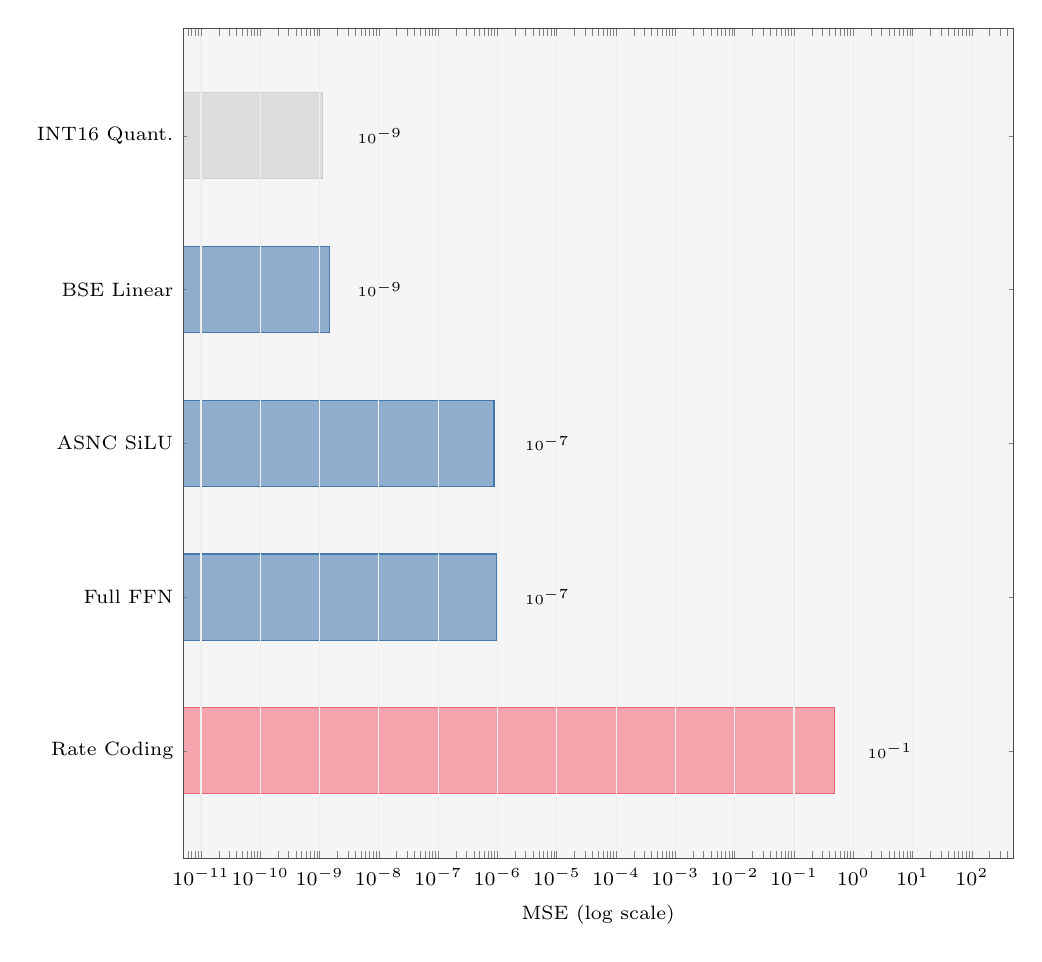
\begin{tikzpicture}
\begin{axis}[
    width=\textwidth,
    height=\textwidth,
    xlabel={\scriptsize MSE (log scale)},
    xmode=log,
    xmin=5e-12, xmax=5e2,
    ymin=0.3, ymax=5.7,
    ytick={1,2,3,4,5},
    yticklabels={
        {\scriptsize INT16 Quant.},
        {\scriptsize BSE Linear},
        {\scriptsize ASNC SiLU},
        {\scriptsize Full FFN},
        {\scriptsize Rate Coding}
    },
    y dir=reverse,
    tick label style={font=\scriptsize},
    label style={font=\scriptsize},
    axis line style={thin, black!70},
    major tick length=1.5pt,
    xmajorgrids=true,
    grid style={TolGrey!25, thin},
    axis on top,
    clip=false,
    axis background/.style={fill=black!4},
]
\fill[TolGrey!50, draw=TolGrey!70]
    (axis cs:5e-12, 0.72) rectangle (axis cs:1.12e-9, 1.28);
\fill[TolBlue!60, draw=TolBlue]
    (axis cs:5e-12, 1.72) rectangle (axis cs:1.45e-9, 2.28);
\fill[TolBlue!60, draw=TolBlue]
    (axis cs:5e-12, 2.72) rectangle (axis cs:8.73e-7, 3.28);
\fill[TolBlue!60, draw=TolBlue]
    (axis cs:5e-12, 3.72) rectangle (axis cs:9.51e-7, 4.28);
\fill[TolRed!60, draw=TolRed]
    (axis cs:5e-12, 4.72) rectangle (axis cs:4.88e-1, 5.28);
\node[font=\tiny, anchor=west] at (axis cs:3e-9, 1)  {$10^{-9}$};
\node[font=\tiny, anchor=west] at (axis cs:3e-9, 2)  {$10^{-9}$};
\node[font=\tiny, anchor=west] at (axis cs:2e-6, 3)  {$10^{-7}$};
\node[font=\tiny, anchor=west] at (axis cs:2e-6, 4)  {$10^{-7}$};
\node[font=\tiny, anchor=west] at (axis cs:1.2e0, 5) {$10^{-1}$};
\end{axis}
\end{tikzpicture}
\label{fig:component_mse}
\end{minipage}
\hfill
\begin{minipage}[c]{0.50\textwidth}
\centering
\small
\begin{tabular}{lc}
\hline
\textbf{FFN Configuration} & \textbf{PPL} \\
\hline
ANN with SiLU (Baseline)       & $5.12 \pm 0.01$ \\
\textit{BSE + Standard SiLU}   & \textit{$5.18 \pm 0.01$} \\
BSE + ReLU                     & $50.74 \pm 0.04$ \\
Rate Coding + ASNC             & $103.5 \pm 10.4$ \\
\textbf{BSE + ASNC (Ours)}     & $\mathbf{5.21 \pm 0.02}$ \\
\hline
\end{tabular}
\label{tab:ffn_force_break}
\end{minipage}
\caption{\textbf{(a)} Component-level MSE on a representative FFN layer (FP16, 16 steps). BSE matches the INT16 floor; ASNC confines error to $10^{-7}$; Rate Coding degrades to $10^{-1}$. \textbf{(b)} System-level PPL confirms: replacing BSE or ASNC with low-fidelity alternatives causes catastrophic degradation; our BSE+ASNC adds only $+0.09$ over the ideal ceiling.}
\end{figure}

\subsubsection{Layer-wise Sensitivity and Progressive SNN-ization}

We next quantify sensitivity by SNN-izing one subsystem at a time, then progressively composing them. Table~\ref{tab:layerwise_ablation} shows that FFN layers are the most sensitive, where replacing them alone increases PPL from $5.12$ to $5.35$ ($+0.23$). Attention layers show a smaller increase to $5.31$, while Embedding and LayerNorm rise by only $+0.08$ and $+0.06$, respectively. Once all subsystems are converted, the final SNN reaches $5.58$, a total increase of $+0.46$. This stepwise pattern confirms that errors add predictably and remain bounded rather than diffusing uncontrollably.

As shown in Table~\ref{tab:progressive_ablation} (right), progressively adding sensitive subsystems makes the accumulation explicit. Starting from FFN-only at $5.35$, adding the nonlinear Activation raises PPL to $5.47$ ($+0.12$), the dominant contribution. The full SNN saturates at $5.61$, less than half a point above baseline.

\begin{table}[h!]
\centering
\caption{Ablation on WikiText-2 perplexity (FP16, 16 steps; baseline PPL\,=\,$5.12\pm0.01$). \textbf{Left:} Layer-wise sensitivity---FFN is the most sensitive ($+0.23$), full SNN ends at $+0.46$. \textbf{Right:} Progressive SNN-ization---errors accumulate additively and remain bounded.}
\label{tab:layerwise_ablation}
\label{tab:progressive_ablation}
\vspace{0.5em}
\begin{minipage}[t]{0.48\textwidth}
\centering
\small
\begin{tabular}{lc}
\hline
\textbf{SNN-ized Component} & \textbf{PPL} \\
\hline
None (Baseline)           & $5.12\pm 0.01$ \\
FFN Layers only           & $5.35 \pm 0.03$ \\
Attention Layers only     & $5.31 \pm 0.02$ \\
Embedding/Output only     & $5.20 \pm 0.02$ \\
LayerNorm only            & $5.18 \pm 0.01$ \\
Full SNN (All)            & $5.58 \pm 0.04$ \\
\hline
\end{tabular}
\end{minipage}
\hfill
\begin{minipage}[t]{0.48\textwidth}
\centering
\small
\begin{tabular}{lc}
\hline
\textbf{Progressive Strategy} & \textbf{PPL} \\
\hline
1.\;FFN only                        & $5.35 \pm 0.03$ \\
2.\;+ Activation                    & $5.47 \pm 0.04$ \\
3.\;+ Attention                     & $5.50 \pm 0.04$ \\
4.\;+ Embedding                     & $5.58 \pm 0.04$ \\
5.\;Full SNN (All)                  & $5.61 \pm 0.04$ \\
\hline
\end{tabular}
\end{minipage}
\end{table}

As shown in Table~\ref{tab:progressive_ablation} (right), progressively adding sensitive subsystems makes the accumulation explicit. Starting from FFN-only at $5.35$, adding the nonlinear Activation raises PPL to $5.47$ ($+0.12$), which accounts for the major increase. Subsequently adding Attention only slightly increases PPL to $5.50$ ($+0.03$). Incorporating Embedding raises it further to $5.58$ ($+0.08$), and finally the Full SNN model results in $5.61$ ($+0.03$). The saturation at less than half a point above baseline demonstrates that errors grow additively but remain tightly bounded, with the dominant contribution coming from the nonlinear Activation.



\subsubsection{Fine-Grained Component Analysis}

We further decompose the sensitive Attention and FFN modules. Within Attention, Table~\ref{tab:attention_fine_grained} indicates that SNN-izing the Q, K, V projections increases PPL by $+0.16$ to $5.28$, whereas converting only the score path adds merely $+0.06$. This shows that linear projections dominate sensitivity, while other operations remain robust.

\begin{table}[h!]
\centering
\caption{PPL analysis (FP16, 16 steps; baseline $5.12\pm0.01$). \textbf{Left:} Attention sub-components---Q/K/V projections raise PPL by $+0.16$, score path adds only $+0.06$. \textbf{Right:} Comparison with SpikeLLM on LLaMA-2 7B---ours is only $+0.46$ above the ANN baseline vs.\ $+6.7$--$+9.0$ for SpikeLLM.}
\label{tab:attention_fine_grained}
\label{tab:spikellm_comparison}
\vspace{0.5em}
\begin{minipage}[t]{0.46\textwidth}
\centering
\small
\begin{tabular}{lc}
\hline
\textbf{Attention Component} & \textbf{PPL} \\
\hline
None (Baseline)       & $5.12\pm 0.01$ \\
QKV Proj. only        & $5.28 \pm 0.03$ \\
Attn Score only       & $5.18 \pm 0.02$ \\
Q+K only              & $5.24 \pm 0.03$ \\
V only                & $5.22 \pm 0.02$ \\
All Attention SNN     & $5.31 \pm 0.05$ \\
\hline
\end{tabular}
\end{minipage}
\hfill
\begin{minipage}[t]{0.50\textwidth}
\centering
\small
\begin{tabular}{lcc}
\hline
\textbf{Method} & \textbf{Quant.} & \textbf{PPL} \\
\hline
ANN Baseline              & FP16  & $5.12$ \\
SpikeLLM                  & W2A16 & $14.16$ \\
SpikeLLM                  & W4A4  & $11.85$ \\
\textbf{Ours (BSE+ASNC)}  & FP16  & $\mathbf{5.58}$ \\
\hline
\end{tabular}
\end{minipage}
\end{table}

For FFN (Figure~\ref{tab:ffn_force_break}b), the gap between our BSE+ASNC and the ideal SiLU ceiling is only $+0.09$ PPL, quantifying the minor fidelity cost introduced by ASNC. In contrast, replacing ASNC with an inconsistent low-fidelity ReLU degrades performance severely to $50.74$ PPL, while replacing BSE with rate coding leads to catastrophic failure beyond $100$ PPL. These results demonstrate that BSE and ASNC are both indispensable for high-fidelity forward propagation.

\subsubsection{Comparison with a Prior Baseline}

As shown in Table~\ref{tab:spikellm_comparison} (right), to contextualize our results we compare against a prior SNN baseline that evaluates spiking variants of LLaMA-2~7B on WikiText-2 under short time-step budgets. Our FP16 ANN baseline achieves a perplexity of $5.12$, while our full SNN (BSE+ASNC, 16 steps) attains $5.58 \pm 0.04$, corresponding to only $+0.46$ higher than the ANN baseline. In contrast, the prior baseline reports perplexities between $11.85$ and $14.16$, i.e., $+6.7$ to $+9.0$ higher than the ANN baseline. Overall, compared to the prior baseline, our method reduces degradation by more than a factor of $2.1$--$2.5\times$, showcasing the significant fidelity advantage of LASER over existing methods in large-scale modeling scenarios.

\begin{table}[h!]
\centering
\caption{Energy ratio of a single ASNC nonlinear operation on Intel Loihi~2 vs.\ SiLU on NVIDIA A100 GPU. Loihi~2 requires only ${\sim}0.5\%$ of GPU energy, a more than $200\times$ reduction.}
\label{tab:hardware_efficiency}
\small
\begin{tabular}{lc}
\hline
\textbf{Precision} & \textbf{Energy Ratio (Loihi~2 / GPU)} \\
\hline
16-bit & $5.5 \times 10^{-3}$ \\
32-bit & $5.3 \times 10^{-3}$ \\
\hline
\end{tabular}
\end{table}

\subsection{End-to-End Performance and Scalability Analysis}
\label{subsec:performance_and_scalability}

We apply our framework to multiple open-source LLMs and report task accuracy under a fixed 16-step budget for SNNs. Table~\ref{tab:sota_scaling_performance_steps_nostyle} shows that across MMLU, HellaSwag, ARC, and TruthfulQA, SNN performance consistently tracks the corresponding ANN baselines. For example, on LLaMA-2 70B, accuracy on MMLU drops by only $1.2\%$ and the overall degradation across all benchmarks remains under $2\%$. On LLaMA-2 7B, perplexity rises by only $+0.46$ compared to the ANN, a negligible difference given the scale of the model. This result demonstrates that the component-level fidelity of BSE and localized error in ASNC carry through to full large-model systems, maintaining near-baseline accuracy under a short, fixed 16-step budget.

% \begin{table}[htbp]
%   \centering
%   \caption{End-to-end performance comparison (accuracy, \%). Across five representative LLMs, accuracy degradation from ANN to SNN remains within $2\%$, with LLaMA-2 70B showing only $-1.2\%$ on MMLU. This confirms that fidelity holds at scale under a fixed 16-step budget. This result demonstrates that when extended to large-scale modeling scenarios, LEASER still maintains high-fidelity forward propagation.
% }
%   \label{tab:sota_scaling_performance_steps_nostyle}
%   \begin{threeparttable}
%   \begin{tabular}{l c cc cc cc cc}
%     \toprule
%     \multirow{2}{*}{Model} & \multirow{2}{*}{Steps} & \multicolumn{2}{c}{MMLU} & \multicolumn{2}{c}{HellaSwag} & \multicolumn{2}{c}{ARC} & \multicolumn{2}{c}{TruthfulQA} \\
%     \cmidrule(lr){3-4} \cmidrule(lr){5-6} \cmidrule(lr){7-8} \cmidrule(lr){9-10}
%      &  & ANN & SNN & ANN & SNN & ANN & SNN & ANN & SNN \\
%     \midrule
%     Phi-2 (2.7B)          & 16 & 58.11 & 56.0 & 75.11 & 72.5 & 61.09 & 58.9 & 44.47 & 42.1 \\
%     Llama-2 (7B)          & 16 & 60.04 & 58.2 & 79.13 & 76.9 & 56.14 & 54.5 & 40.95 & 39.0 \\
%     Mistral (7.3B)        & 16 & 60.78 & 59.1 & 84.88 & 83.0 & 63.14 & 61.5 & 68.26 & 66.0 \\
%     Mistral (8$\times$7B) & 16 & 68.59 & 68.0 & 86.03 & 85.2 & 67.24 & 66.5 & 59.54 & 58.3 \\
%     Llama-2 (70B)         & 16 & 65.40 & 64.2 & 86.90 & 85.5 & 67.20 & 65.8 & 44.90 & 43.1 \\
%     \bottomrule
%   \end{tabular}
%   \end{threeparttable}
% \end{table}

\begin{table}[h!]
  \centering
  \caption{End-to-end performance comparison (accuracy, \%; all SNNs use FP16 with a fixed 16-step budget). Degradation from ANN to SNN remains within $2\%$ across all benchmarks, with LLaMA-2 70B showing only $-1.2\%$ on MMLU.}
  \label{tab:sota_scaling_performance_steps_nostyle}
  \small
    \begin{tabular*}{\textwidth}{@{\extracolsep{\fill}}l cc cc cc cc}
      \toprule
      \multirow{2}{*}{Model} & \multicolumn{2}{c}{MMLU} & \multicolumn{2}{c}{HellaSwag} & \multicolumn{2}{c}{ARC} & \multicolumn{2}{c}{TruthfulQA} \\
      \cmidrule(lr){2-3} \cmidrule(lr){4-5} \cmidrule(lr){6-7} \cmidrule(lr){8-9}
        & ANN & SNN & ANN & SNN & ANN & SNN & ANN & SNN \\
      \midrule
      Phi-2 (2.7B)          & 58.11 & 56.0 & 75.11 & 72.5 & 61.09 & 58.9 & 44.47 & 42.1 \\
      Llama-2 (7B)          & 60.04 & 58.2 & 79.13 & 76.9 & 56.14 & 54.5 & 40.95 & 39.0 \\
      Mistral (7.3B)        & 60.78 & 59.1 & 84.88 & 83.0 & 63.14 & 61.5 & 68.26 & 66.0 \\
      Mistral (8$\times$7B) & 68.59 & 68.0 & 86.03 & 85.2 & 67.24 & 66.5 & 59.54 & 58.3 \\
      Llama-2 (70B)         & 65.40 & 64.2 & 86.90 & 85.5 & 67.20 & 65.8 & 44.90 & 43.1 \\
      \bottomrule
    \end{tabular*}
\end{table}
\subsection{Empirical Analysis of Energy Efficiency on Neuromorphic Hardware}
\label{subsec:hardware_efficiency_analysis}

We finally examine energy in practice by benchmarking the core nonlinear component on Intel Loihi~2 and comparing against an ANN SiLU baseline on an NVIDIA A100 under matched precisions. Loihi~2 energy per operation is obtained from on-board probes. GPU energy per operation is estimated from sustained-load power measurements over millions of identical operations using \texttt{nvidia-smi}. As shown in Table~\ref{tab:hardware_efficiency}, Loihi~2 consumes only about $0.5\%$ of the GPU energy at both 16-bit and 32-bit settings, representing more than a $200\times$ reduction. Together with the earlier accuracy results showing less than $2\%$ loss at scale, this demonstrates that the proposed design achieves substantial energy savings while preserving near-baseline accuracy, consistent with our roadmap toward precise, scalable SNNs.

% [Hardware efficiency table merged into Table with spikellm_comparison above]

\section{Conclusion}
\label{sec:conclusion}
% LASER 构建了一个三步路线：BSE 保证线性计算严格等价，ASNC 将近似误差局限于唯一的非线性模块，而在这一高保真且结构一致的前向传播基础上，引入轻量的恒等梯度 STE 能够实现稳定可控的训练。实验结果表明，BSE 在编码上达到机器级精度，ASNC 的误差仅出现在单一可量化点上，STE 则在全局范围内保持稳定且无扩散。在 LLaMA-2 70B 上，MMLU 准确率仅下降 1.2%，而在 LLaMA-2 7B 上困惑度仅增加 +0.46。结合在 Loihi 2 上实现的约 200 倍能效提升，这些结果表明 LASER 在大规模脉冲模型中统一了高保真、可控性与可扩展性。
LASER\textendash SNN establishes a three\textendash step roadmap: BSE guarantees strict equivalence in linear computations, ASNC confines approximation error to a single nonlinear module, and—on this high\textendash fidelity, structurally consistent forward path—a lightweight identity\textendash gradient STE enables stable and controllable training. Experimental results demonstrate that BSE achieves machine\textendash level precision in encoding, ASNC introduces error only at one quantifiable point, and STE maintains stability without diffusion. On \mbox{LLaMA\textendash 2} 70B, accuracy on MMLU decreases by merely 1.2\%, while on \mbox{LLaMA\textendash 2} 7B, perplexity increases by only {+}0.46. Combined with a $200\times$ improvement in energy efficiency on Loihi~2, these results show that LASER\textendash SNN unifies fidelity, controllability, and scalability in large\textendash scale spiking models.

\bibliographystyle{plainnat}
\bibliography{references}

%%%%%%%%%%%%%%%%%%%%%%%%%%%%%%%%%%%%%%%%%%%%%%%%%%%%%%%%%%%%%%%%%%%%%%%%%%%%%%%
% APPENDIX
%%%%%%%%%%%%%%%%%%%%%%%%%%%%%%%%%%%%%%%%%%%%%%%%%%%%%%%%%%%%%%%%%%%%%%%%%%%%%%%
\appendix
\section{Entropy Preservation of BSE}
\label{app:bse_entropy_proof}

\paragraph{Setting.}
Fix a bit-window length $N\in\mathbb{N}$. For each channel, let the per-layer affine calibration be $(\lambda,\mu)$ with $\lambda>0$ and $\mu\in\mathbb{R}$. Define the $N$-bit quantizer
\begin{equation}
\label{eq:quantizer_grid_def}
\mathcal{Q}_N \;\triangleq\; \{0,1,\dots,2^{N}-1\}, 
\qquad 
q \;=\; \mathrm{clip}_{[0,\,2^N-1]}\!\Big(\mathrm{round}\big(\lambda\,(x+\mu)\big)\Big).
\end{equation}
The corresponding de-quantization (reconstruction) map is $\hat{x}=\lambda^{-1}q-\mu$.
Write the binary expansion of $q$ as
\begin{equation}
\label{eq:binary_expansion_def}
q \;=\; \sum_{t=0}^{N-1} b_t\,2^{N-1-t},
\qquad b_t\in\{0,1\}.
\end{equation}

\paragraph{BSE encoder/decoder.}
Let the bit-weights and thresholds be the standard positional schedule
\begin{equation}
\label{eq:standard_bit_schedule}
W_{\mathrm{bit}}(t) \;=\; 2^{\,N-1-t},
\qquad 
\Theta(t) \;=\; W_{\mathrm{bit}}(t),
\qquad t=0,\dots,N-1.
\end{equation}
Drive the non-leaky IF unit \eqref{eq:if_forward_clean} with a single impulse carrying the integer code:
\begin{equation}
\label{eq:scalar_drive}
I_{\mathrm{in}}(t) \;=\; \delta_{t0}\,q,
\qquad 
V_m(0)=0.
\end{equation}
The \emph{BSE encoder} $\mathsf{E}_N:\mathcal{Q}_N\to\{0,1\}^{N}$ is defined as the spike train $S(t)\equiv S_{\mathrm{actual}}(t)$ produced by \eqref{eq:if_forward_clean}, $t=0,\dots,N-1$. The \emph{BSE decoder} $\mathsf{D}_N:\{0,1\}^{N}\to\mathcal{Q}_N$ is the weighted sum
\begin{equation}
\label{eq:bse_decoder}
\mathsf{D}_N\big(\{s(t)\}_{t=0}^{N-1}\big) \;=\; \sum_{t=0}^{N-1} s(t)\,2^{\,N-1-t}.
\end{equation}

\begin{lemma}[Bit-exact emission]
\label{lem:bit_exact}
Under \eqref{eq:standard_bit_schedule}–\eqref{eq:scalar_drive}, the encoder emits the binary digits of $q$ in MSB$\to$LSB order:
\[
S(t)\;=\;b_t\quad\text{for all }t=0,\dots,N-1,
\]
and the membrane obeys $V_m(t)=\sum_{\tau>t} b_\tau\,2^{\,N-1-\tau}$ for $t=0,\dots,N$ (with the empty sum $0$ at $t=N$).
\end{lemma}

\begin{proof}
By \eqref{eq:if_forward_clean} and \eqref{eq:scalar_drive},
\[
V_m(0)=0,\quad V_m(0)+I_{\mathrm{in}}(0)=q.
\]
At $t=0$ the threshold is $\Theta(0)=2^{N-1}$. Hence $M_0=\mathbb{1}\{q\ge 2^{N-1}\}=b_0$ and the post-update membrane is
\[
V_m(1)=q-b_0\,2^{N-1}=\sum_{\tau=1}^{N-1} b_\tau\,2^{\,N-1-\tau}.
\]
Assume the claim holds up to time $t$. Then $V_m(t)=\sum_{\tau>t} b_\tau\,2^{N-1-\tau}$ and $\Theta(t)=2^{N-1-t}$. Thus
\[
M_t=\mathbb{1}\{V_m(t)\ge \Theta(t)\}=\mathbb{1}\Big\{\sum_{\tau>t} b_\tau\,2^{N-1-\tau}\ \ge\ 2^{N-1-t}\Big\}=b_t,
\]
since the sum's leading term is $b_t\,2^{N-1-t}$ and all lower-order terms are strictly smaller than $2^{N-1-t}$. The update gives
\[
V_m(t+1)=V_m(t)-M_t\,\Theta(t)=\sum_{\tau>t} b_\tau\,2^{N-1-\tau}-b_t\,2^{N-1-t}=\sum_{\tau>t+1} b_\tau\,2^{N-1-\tau}.
\]
By induction the statements hold for all $t$, and $V_m(N)=0$.
\end{proof}

\begin{theorem}[Encoder–decoder bijection]
\label{thm:bijective}
$\mathsf{E}_N$ and $\mathsf{D}_N$ are mutual inverses:
\[
\mathsf{D}_N\big(\mathsf{E}_N(q)\big)=q\quad\text{for all }q\in\mathcal{Q}_N,
\qquad
\mathsf{E}_N\big(\mathsf{D}_N(S)\big)=S\quad\text{for all }S\in\{0,1\}^{N}.
\]
\end{theorem}

\begin{proof}
The first identity follows from Lemma~\ref{lem:bit_exact} and \eqref{eq:bse_decoder}:
\[
\mathsf{D}_N\big(\mathsf{E}_N(q)\big)=\sum_{t=0}^{N-1} S(t)\,2^{N-1-t}=\sum_{t=0}^{N-1} b_t\,2^{N-1-t}=q.
\]
For the second identity, any $S\in\{0,1\}^N$ defines $q^\star=\mathsf{D}_N(S)$ with binary digits $b_t^\star=S(t)$. Lemma~\ref{lem:bit_exact} shows that driving the IF with $q^\star$ emits $b_t^\star$ at time $t$, i.e., $\mathsf{E}_N(q^\star)=S$.
\end{proof}

\begin{theorem}[Entropy preservation at $N$-bit alignment]
\label{thm:entropy_preservation}
Let $X$ be any real-valued random variable and let $Q=\mathrm{clip}\!\circ\!\mathrm{round}(\lambda(X+\mu))\in\mathcal{Q}_N$ be its $N$-bit quantization \eqref{eq:quantizer_grid_def}. Let $S=\mathsf{E}_N(Q)$ be the BSE spike code under \eqref{eq:standard_bit_schedule}–\eqref{eq:scalar_drive}. Then the (discrete) Shannon entropy is invariant:
\[
H(Q)=H(S).
\]
Equivalently, the pushforward distribution on spike sequences is a relabeling of the code distribution.
\end{theorem}

\begin{proof}
By Theorem~\ref{thm:bijective}, $\mathsf{E}_N$ is a bijection between the finite sets $\mathcal{Q}_N$ and $\{0,1\}^{N}$. Hence, for all $s\in\{0,1\}^{N}$,
\[
\mathbb{P}[S=s]=\mathbb{P}\big[Q=\mathsf{D}_N(s)\big].
\]
Therefore
\[
H(S)=-\sum_{s}\mathbb{P}[S=s]\log \mathbb{P}[S=s]
=-\sum_{q}\mathbb{P}[Q=q]\log \mathbb{P}[Q=q]=H(Q).
\]
\end{proof}

\paragraph{Vector/batch case.}
For $B$ samples and $d$ channels, define $Q\in\mathcal{Q}_N^{B\times d}$ and $S\in\{0,1\}^{N\times B\times d}$ by applying $(\lambda,\mu)$ per channel and $\mathsf{E}_N$ elementwise. The map $\mathsf{E}_N^{\otimes Bd}$ is a bijection between the two finite sets, so the joint entropy is preserved:
\[
H\big(Q_{1:B,1:d}\big)=H\big(S_{0:N-1,\,1:B,\,1:d}\big).
\]

\paragraph{Exactness of spike-domain accumulation.}
Within a bit window, the Soma pre-accumulation equals decoding in \eqref{eq:bse_decoder}:
\[
Q_a \;=\; \sum_{t=0}^{N-1} S_a(t)\,W_{\mathrm{bit}}(t),
\]
so for any weight matrix $W$ the linear map $A=Q_a W^\top$ is identical to applying $W$ to the decoded integers. Thus all spike-domain accumulations are \emph{exact integer arithmetic}. The only approximation in the BSE pathway appears at the explicit rounding/clipping that defines $Q$ (or $Q_y$ in \eqref{eq:soma_def}).

\begin{corollary}[No error diffusion from BSE under $N$-bit alignment]
\label{cor:no_diffusion}
Assume each layer uses $(\lambda,\mu)$ that matches its $N$-bit quantization grid and uses the binary schedule \eqref{eq:standard_bit_schedule}. Then, relative to the corresponding $N$-bit quantized ANN, the BSE forward is functionally identical: encoding, spike-domain accumulation, and decoding are exact and introduce \emph{no additional error}. Consequently, any discrepancy from full precision equals the ANN's own $N$-bit quantization error and does not diffuse or amplify due to BSE.
\end{corollary}

\paragraph{Remarks.}
(i) The proof only requires a positional system with unique representation; the binary schedule \eqref{eq:standard_bit_schedule} is the canonical choice.  
(ii) Signed ranges are handled by the offset $\mu$ (cf.\ \eqref{eq:soma_def}), which translates the dynamic range to $[0,2^N-1]$ before encoding and back after decoding; bijectivity and entropy preservation hold channelwise under this affine change of variables.  
(iii) The results extend verbatim to per-channel $(\lambda_o,\mu_o)$ and per-layer bit windows, provided $N$ is the operative grid width used by the ANN baseline.

\section{Proof of ASNC Error Bound Superiority}
\label{app:asnc_proof}

\subsection{Setup}
Let $X \sim \mathcal N(0,1)$ and consider only the nonnegative half-axis $[0,\infty)$, which corresponds to the effective input of ReLU-type nonlinearities.  
We partition the input space into $n$ intervals and approximate the nonlinear response by piecewise-constant reconstruction points $\{y_i\}_{i=1}^n$.  
The mean squared error (MSE) distortion is defined as
\[
D_n = \mathbb{E}\big[(X - Q_n(X))^2\big].
\]

\subsection{Non-uniform Quantization Error Bound}
According to Bennett's integral and Lloyd–Max theory \citep{gersho1992vector}, for any continuous density $f$ with finite second moment, the high-rate distortion of the optimal non-uniform quantizer is
\[
D_n^{\text{non-uniform}}
= \frac{1}{12}\,n^{-2}\left(\int_{0}^{\infty} f(x)^{1/3}\,dx\right)^3 + o(n^{-2}), \quad n \to \infty.
\]
For Gaussian input $f(x)$, the integral is finite and well-defined, giving the asymptotic error constant $C_{\text{non-uniform}}$.

\subsection{Uniform Partitioning Error Bound (e.g., SpikeZIP-FT)}
Consider a uniform quantization scheme, such as SpikeZIP-FT \citep{you2024spikeziptf}, which partitions the truncated interval $[0,R]$ into $n$ equal subintervals of width $\Delta = R/n$.  
The corresponding distortion is
\[
D_n^{\text{uniform}} 
= \frac{1}{12}\,\Delta^2 \sum_{i=1}^n \Pr(X \in I_i) 
   + \int_{R}^{\infty} (x-R)^2 f(x)\,dx .
\]
Choosing $R = \Theta(\sqrt{\log n})$ makes the tail term negligible, yielding the asymptotic form
\[
D_n^{\text{uniform}} 
= \frac{R^2}{12n^2}\int_{0}^{\infty} f(x)\,dx + o(n^{-2}).
\]
This defines the uniform error constant $C_{\text{uniform}}$.

\subsection{Comparison and Conclusion}
By Hölder’s inequality, for any non-constant density $f$, 
\[
\Big(\int f^{1/3}(x)\,dx\Big)^3 < R^2 \int f(x)\,dx .
\]
For Gaussian $f(x)$ this inequality is strict. Hence,
\[
C_{\text{non-uniform}} < C_{\text{uniform}}.
\]

\paragraph{Conclusion.}  
For Gaussian inputs, ASNC (non-uniform partitioning) achieves a strictly smaller asymptotic error bound than uniform partitioning methods such as SpikeZIP-FT. Therefore, under the same number of intervals $n$, the error of ASNC satisfies
\[
D_n^{\text{ASNC}} < D_n^{\text{SpikeZIP-FT}} .
\]
This establishes the theoretical advantage of ASNC in terms of error–latency tradeoff.


\section{ASNC Formal Specification}
\label{app:asnc_details}

\subsection{Segmental Codec and BSE Re-encoding}
\paragraph{Core Objective.}
Each segmental codec $\mathcal{C}_i(x)$ utilizes a spiking neural structure:
\begin{align}
\text{spikes}_i(t) &= \mathrm{LIF}\!\big(\mathrm{quantize}(x\, s_i + b_i),\, \theta_i(t)\big), \\
\mathcal{C}_i(x) &= \sum_{t=1}^{T} w_i(t)\, \text{spikes}_i(t),
\end{align}
where $w_i(t)$ are trainable decoding weights for segment $i$.

\paragraph{BSE-Compatible Output.}
The decoded analog value $\widehat{y}_i$ for each active segment is immediately re-encoded by the BSE encoder to produce $S^{\mathrm{BSE}}_i(t)$ within the same window $T$; the overall output is
\begin{equation}
S^{\mathrm{BSE}}(t) \;=\; \sum_{i=1}^{N} \mathcal{I}_i(x)\, S^{\mathrm{BSE}}_i(t).
\end{equation}

\subsection{Adaptive Splitting Algorithm}
\paragraph{Split Criterion.}
\begin{equation}
\frac{L_i}{\bar{L}} \cdot \big(1 + \sigma_i^2\big) \cdot \rho_i \;>\; \tau_{\mathrm{adaptive}}.
\end{equation}

\paragraph{Adaptive Threshold.}
\begin{equation}
\tau_{\mathrm{adaptive}} \;=\; \tau_{\mathrm{base}} \cdot \alpha_{\mathrm{stag}} \cdot \alpha_{\mathrm{prog}},
\end{equation}
where $\tau_{\mathrm{base}}$ is a base threshold, and $\alpha$ factors correct for stagnation and training progress.

\paragraph{Stagnation Factor $\alpha_{\mathrm{stag}}$.}
\begin{equation}
\alpha_{\mathrm{stag}} \;=\;
\begin{cases}
0.2, & \text{if } N_{\mathrm{stag}}/N_{\mathrm{active}} > 0.6,\\
0.4, & \text{if } N_{\mathrm{stag}}/N_{\mathrm{active}} > 0.3,\\
1.0, & \text{otherwise.}
\end{cases}
\end{equation}

\paragraph{Progress Factor $\alpha_{\mathrm{prog}}$.}
\begin{equation}
\alpha_{\mathrm{prog}} \;=\;
\begin{cases}
0.4, & \text{if } (L_0 - L_t)/L_0 < 0.005,\\
0.6, & \text{if } (L_0 - L_t)/L_0 < 0.02,\\
1.0, & \text{otherwise.}
\end{cases}
\end{equation}

\paragraph{Split Point Selection.}
\begin{align}
S(x_s) \;=\; \alpha_1\, E_{\mathrm{sep}}(x_s) \;+\; \alpha_2\, C_{\mathrm{cons}}(x_s)
\;+\; \alpha_3\, B_{\mathrm{bal}}(x_s) \;+\; \alpha_4\, Y_{\mathrm{sep}}(x_s).
\end{align}

\subsection{Adaptive Weighting Mechanism}
\paragraph{Morphology-Aware Weights.}
\begin{equation}
w_i \;=\; 0.5\, I_{\mathrm{func}}(i) \;+\; 0.35\, I_{\mathrm{error}}(i) \;+\; 0.15\, D_i.
\end{equation}
\paragraph{Regional Priority $R_{\mathrm{region}}(i)$.}
\begin{equation}
R_{\mathrm{region}}(i) \;=\;
\begin{cases}
3.0, & a_i < 0 \text{ and } b_i > 0 \quad \text{(Zero-Crossing Region)},\\
2.5, & b_i \le 0 \quad \text{(Purely Negative Region)},\\
2.0, & a_i \ge 0 \quad \text{(Purely Positive Region)},\\
1.0, & \text{otherwise.}
\end{cases}
\end{equation}

%%%%%%%%%%%%%%%%%%%%%%%%%%%%%%%%%%%%%%%%%%%%%%%%%%%%%%%%%%%%%%%%%%%%%%%%%%%%%%%
% CHECKLIST
%%%%%%%%%%%%%%%%%%%%%%%%%%%%%%%%%%%%%%%%%%%%%%%%%%%%%%%%%%%%%%%%%%%%%%%%%%%%%%%
\newpage
\section*{NeurIPS Paper Checklist}

%%% BEGIN INSTRUCTIONS %%%
The checklist is designed to encourage best practices for responsible machine learning research, addressing issues of reproducibility, transparency, research ethics, and societal impact. Do not remove the checklist: {\bf The papers not including the checklist will be desk rejected.} The checklist should follow the references and follow the (optional) supplemental material.  The checklist does NOT count towards the page
limit. 

Please read the checklist guidelines carefully for information on how to answer these questions. For each question in the checklist:
\begin{itemize}
    \item You should answer \answerYes{}, \answerNo{}, or \answerNA{}.
    \item \answerNA{} means either that the question is Not Applicable for that particular paper or the relevant information is Not Available.
    \item Please provide a short (1--2 sentence) justification right after your answer (even for \answerNA). 
   % \item {\bf The papers not including the checklist will be desk rejected.}
\end{itemize}

{\bf The checklist answers are an integral part of your paper submission.} They are visible to the reviewers, area chairs, senior area chairs, and ethics reviewers. You will also be asked to include it (after eventual revisions) with the final version of your paper, and its final version will be published with the paper.

The reviewers of your paper will be asked to use the checklist as one of the factors in their evaluation. While \answerYes{} is generally preferable to \answerNo{}, it is perfectly acceptable to answer \answerNo{} provided a proper justification is given (e.g., error bars are not reported because it would be too computationally expensive'' or ``we were unable to find the license for the dataset we used''). In general, answering \answerNo{} or \answerNA{} is not grounds for rejection. While the questions are phrased in a binary way, we acknowledge that the true answer is often more nuanced, so please just use your best judgment and write a justification to elaborate. All supporting evidence can appear either in the main paper or the supplemental material, provided in appendix. If you answer \answerYes{} to a question, in the justification please point to the section(s) where related material for the question can be found.

IMPORTANT, please:
\begin{itemize}
    \item {\bf Delete this instruction block, but keep the section heading ``NeurIPS Paper Checklist"},
    \item  {\bf Keep the checklist subsection headings, questions/answers and guidelines below.}
    \item {\bf Do not modify the questions and only use the provided macros for your answers}.
\end{itemize} 
 

%%% END INSTRUCTIONS %%%


\begin{enumerate}

\item {\bf Claims}
    \item[] Question: Do the main claims made in the abstract and introduction accurately reflect the paper's contributions and scope?
    \item[] Answer: \answerTODO{} % Replace by \answerYes{}, \answerNo{}, or \answerNA{}.
    \item[] Justification: \justificationTODO{}
    \item[] Guidelines:
    \begin{itemize}
        \item The answer \answerNA{} means that the abstract and introduction do not include the claims made in the paper.
        \item The abstract and/or introduction should clearly state the claims made, including the contributions made in the paper and important assumptions and limitations. A \answerNo{} or \answerNA{} answer to this question will not be perceived well by the reviewers. 
        \item The claims made should match theoretical and experimental results, and reflect how much the results can be expected to generalize to other settings. 
        \item It is fine to include aspirational goals as motivation as long as it is clear that these goals are not attained by the paper. 
    \end{itemize}

\item {\bf Limitations}
    \item[] Question: Does the paper discuss the limitations of the work performed by the authors?
    \item[] Answer: \answerTODO{} % Replace by \answerYes{}, \answerNo{}, or \answerNA{}.
    \item[] Justification: \justificationTODO{}
    \item[] Guidelines:
    \begin{itemize}
        \item The answer \answerNA{} means that the paper has no limitation while the answer \answerNo{} means that the paper has limitations, but those are not discussed in the paper. 
        \item The authors are encouraged to create a separate ``Limitations'' section in their paper.
        \item The paper should point out any strong assumptions and how robust the results are to violations of these assumptions (e.g., independence assumptions, noiseless settings, model well-specification, asymptotic approximations only holding locally). The authors should reflect on how these assumptions might be violated in practice and what the implications would be.
        \item The authors should reflect on the scope of the claims made, e.g., if the approach was only tested on a few datasets or with a few runs. In general, empirical results often depend on implicit assumptions, which should be articulated.
        \item The authors should reflect on the factors that influence the performance of the approach. For example, a facial recognition algorithm may perform poorly when image resolution is low or images are taken in low lighting. Or a speech-to-text system might not be used reliably to provide closed captions for online lectures because it fails to handle technical jargon.
        \item The authors should discuss the computational efficiency of the proposed algorithms and how they scale with dataset size.
        \item If applicable, the authors should discuss possible limitations of their approach to address problems of privacy and fairness.
        \item While the authors might fear that complete honesty about limitations might be used by reviewers as grounds for rejection, a worse outcome might be that reviewers discover limitations that aren't acknowledged in the paper. The authors should use their best judgment and recognize that individual actions in favor of transparency play an important role in developing norms that preserve the integrity of the community. Reviewers will be specifically instructed to not penalize honesty concerning limitations.
    \end{itemize}

\item {\bf Theory assumptions and proofs}
    \item[] Question: For each theoretical result, does the paper provide the full set of assumptions and a complete (and correct) proof?
    \item[] Answer: \answerTODO{} % Replace by \answerYes{}, \answerNo{}, or \answerNA{}.
    \item[] Justification: \justificationTODO{}
    \item[] Guidelines:
    \begin{itemize}
        \item The answer \answerNA{} means that the paper does not include theoretical results. 
        \item All the theorems, formulas, and proofs in the paper should be numbered and cross-referenced.
        \item All assumptions should be clearly stated or referenced in the statement of any theorems.
        \item The proofs can either appear in the main paper or the supplemental material, but if they appear in the supplemental material, the authors are encouraged to provide a short proof sketch to provide intuition. 
        \item Inversely, any informal proof provided in the core of the paper should be complemented by formal proofs provided in appendix or supplemental material.
        \item Theorems and Lemmas that the proof relies upon should be properly referenced. 
    \end{itemize}

    \item {\bf Experimental result reproducibility}
    \item[] Question: Does the paper fully disclose all the information needed to reproduce the main experimental results of the paper to the extent that it affects the main claims and/or conclusions of the paper (regardless of whether the code and data are provided or not)?
    \item[] Answer: \answerTODO{} % Replace by \answerYes{}, \answerNo{}, or \answerNA{}.
    \item[] Justification: \justificationTODO{}
    \item[] Guidelines:
    \begin{itemize}
        \item The answer \answerNA{} means that the paper does not include experiments.
        \item If the paper includes experiments, a \answerNo{} answer to this question will not be perceived well by the reviewers: Making the paper reproducible is important, regardless of whether the code and data are provided or not.
        \item If the contribution is a dataset and\slash or model, the authors should describe the steps taken to make their results reproducible or verifiable. 
        \item Depending on the contribution, reproducibility can be accomplished in various ways. For example, if the contribution is a novel architecture, describing the architecture fully might suffice, or if the contribution is a specific model and empirical evaluation, it may be necessary to either make it possible for others to replicate the model with the same dataset, or provide access to the model. In general. releasing code and data is often one good way to accomplish this, but reproducibility can also be provided via detailed instructions for how to replicate the results, access to a hosted model (e.g., in the case of a large language model), releasing of a model checkpoint, or other means that are appropriate to the research performed.
        \item While NeurIPS does not require releasing code, the conference does require all submissions to provide some reasonable avenue for reproducibility, which may depend on the nature of the contribution. For example
        \begin{enumerate}
            \item If the contribution is primarily a new algorithm, the paper should make it clear how to reproduce that algorithm.
            \item If the contribution is primarily a new model architecture, the paper should describe the architecture clearly and fully.
            \item If the contribution is a new model (e.g., a large language model), then there should either be a way to access this model for reproducing the results or a way to reproduce the model (e.g., with an open-source dataset or instructions for how to construct the dataset).
            \item We recognize that reproducibility may be tricky in some cases, in which case authors are welcome to describe the particular way they provide for reproducibility. In the case of closed-source models, it may be that access to the model is limited in some way (e.g., to registered users), but it should be possible for other researchers to have some path to reproducing or verifying the results.
        \end{enumerate}
    \end{itemize}


\item {\bf Open access to data and code}
    \item[] Question: Does the paper provide open access to the data and code, with sufficient instructions to faithfully reproduce the main experimental results, as described in supplemental material?
    \item[] Answer: \answerTODO{} % Replace by \answerYes{}, \answerNo{}, or \answerNA{}.
    \item[] Justification: \justificationTODO{}
    \item[] Guidelines:
    \begin{itemize}
        \item The answer \answerNA{} means that paper does not include experiments requiring code.
        \item Please see the NeurIPS code and data submission guidelines (\url{https://neurips.cc/public/guides/CodeSubmissionPolicy}) for more details.
        \item While we encourage the release of code and data, we understand that this might not be possible, so \answerNo{} is an acceptable answer. Papers cannot be rejected simply for not including code, unless this is central to the contribution (e.g., for a new open-source benchmark).
        \item The instructions should contain the exact command and environment needed to run to reproduce the results. See the NeurIPS code and data submission guidelines (\url{https://neurips.cc/public/guides/CodeSubmissionPolicy}) for more details.
        \item The authors should provide instructions on data access and preparation, including how to access the raw data, preprocessed data, intermediate data, and generated data, etc.
        \item The authors should provide scripts to reproduce all experimental results for the new proposed method and baselines. If only a subset of experiments are reproducible, they should state which ones are omitted from the script and why.
        \item At submission time, to preserve anonymity, the authors should release anonymized versions (if applicable).
        \item Providing as much information as possible in supplemental material (appended to the paper) is recommended, but including URLs to data and code is permitted.
    \end{itemize}


\item {\bf Experimental setting/details}
    \item[] Question: Does the paper specify all the training and test details (e.g., data splits, hyperparameters, how they were chosen, type of optimizer) necessary to understand the results?
    \item[] Answer: \answerTODO{} % Replace by \answerYes{}, \answerNo{}, or \answerNA{}.
    \item[] Justification: \justificationTODO{}
    \item[] Guidelines:
    \begin{itemize}
        \item The answer \answerNA{} means that the paper does not include experiments.
        \item The experimental setting should be presented in the core of the paper to a level of detail that is necessary to appreciate the results and make sense of them.
        \item The full details can be provided either with the code, in appendix, or as supplemental material.
    \end{itemize}

\item {\bf Experiment statistical significance}
    \item[] Question: Does the paper report error bars suitably and correctly defined or other appropriate information about the statistical significance of the experiments?
    \item[] Answer: \answerTODO{} % Replace by \answerYes{}, \answerNo{}, or \answerNA{}.
    \item[] Justification: \justificationTODO{}
    \item[] Guidelines:
    \begin{itemize}
        \item The answer \answerNA{} means that the paper does not include experiments.
        \item The authors should answer \answerYes{} if the results are accompanied by error bars, confidence intervals, or statistical significance tests, at least for the experiments that support the main claims of the paper.
        \item The factors of variability that the error bars are capturing should be clearly stated (for example, train/test split, initialization, random drawing of some parameter, or overall run with given experimental conditions).
        \item The method for calculating the error bars should be explained (closed form formula, call to a library function, bootstrap, etc.)
        \item The assumptions made should be given (e.g., Normally distributed errors).
        \item It should be clear whether the error bar is the standard deviation or the standard error of the mean.
        \item It is OK to report 1-sigma error bars, but one should state it. The authors should preferably report a 2-sigma error bar than state that they have a 96\% CI, if the hypothesis of Normality of errors is not verified.
        \item For asymmetric distributions, the authors should be careful not to show in tables or figures symmetric error bars that would yield results that are out of range (e.g., negative error rates).
        \item If error bars are reported in tables or plots, the authors should explain in the text how they were calculated and reference the corresponding figures or tables in the text.
    \end{itemize}

\item {\bf Experiments compute resources}
    \item[] Question: For each experiment, does the paper provide sufficient information on the computer resources (type of compute workers, memory, time of execution) needed to reproduce the experiments?
    \item[] Answer: \answerTODO{} % Replace by \answerYes{}, \answerNo{}, or \answerNA{}.
    \item[] Justification: \justificationTODO{}
    \item[] Guidelines:
    \begin{itemize}
        \item The answer \answerNA{} means that the paper does not include experiments.
        \item The paper should indicate the type of compute workers CPU or GPU, internal cluster, or cloud provider, including relevant memory and storage.
        \item The paper should provide the amount of compute required for each of the individual experimental runs as well as estimate the total compute. 
        \item The paper should disclose whether the full research project required more compute than the experiments reported in the paper (e.g., preliminary or failed experiments that didn't make it into the paper). 
    \end{itemize}
    
\item {\bf Code of ethics}
    \item[] Question: Does the research conducted in the paper conform, in every respect, with the NeurIPS Code of Ethics \url{https://neurips.cc/public/EthicsGuidelines}?
    \item[] Answer: \answerTODO{} % Replace by \answerYes{}, \answerNo{}, or \answerNA{}.
    \item[] Justification: \justificationTODO{}
    \item[] Guidelines:
    \begin{itemize}
        \item The answer \answerNA{} means that the authors have not reviewed the NeurIPS Code of Ethics.
        \item If the authors answer \answerNo, they should explain the special circumstances that require a deviation from the Code of Ethics.
        \item The authors should make sure to preserve anonymity (e.g., if there is a special consideration due to laws or regulations in their jurisdiction).
    \end{itemize}


\item {\bf Broader impacts}
    \item[] Question: Does the paper discuss both potential positive societal impacts and negative societal impacts of the work performed?
    \item[] Answer: \answerTODO{} % Replace by \answerYes{}, \answerNo{}, or \answerNA{}.
    \item[] Justification: \justificationTODO{}
    \item[] Guidelines:
    \begin{itemize}
        \item The answer \answerNA{} means that there is no societal impact of the work performed.
        \item If the authors answer \answerNA{} or \answerNo, they should explain why their work has no societal impact or why the paper does not address societal impact.
        \item Examples of negative societal impacts include potential malicious or unintended uses (e.g., disinformation, generating fake profiles, surveillance), fairness considerations (e.g., deployment of technologies that could make decisions that unfairly impact specific groups), privacy considerations, and security considerations.
        \item The conference expects that many papers will be foundational research and not tied to particular applications, let alone deployments. However, if there is a direct path to any negative applications, the authors should point it out. For example, it is legitimate to point out that an improvement in the quality of generative models could be used to generate Deepfakes for disinformation. On the other hand, it is not needed to point out that a generic algorithm for optimizing neural networks could enable people to train models that generate Deepfakes faster.
        \item The authors should consider possible harms that could arise when the technology is being used as intended and functioning correctly, harms that could arise when the technology is being used as intended but gives incorrect results, and harms following from (intentional or unintentional) misuse of the technology.
        \item If there are negative societal impacts, the authors could also discuss possible mitigation strategies (e.g., gated release of models, providing defenses in addition to attacks, mechanisms for monitoring misuse, mechanisms to monitor how a system learns from feedback over time, improving the efficiency and accessibility of ML).
    \end{itemize}
    
\item {\bf Safeguards}
    \item[] Question: Does the paper describe safeguards that have been put in place for responsible release of data or models that have a high risk for misuse (e.g., pre-trained language models, image generators, or scraped datasets)?
    \item[] Answer: \answerTODO{} % Replace by \answerYes{}, \answerNo{}, or \answerNA{}.
    \item[] Justification: \justificationTODO{}
    \item[] Guidelines:
    \begin{itemize}
        \item The answer \answerNA{} means that the paper poses no such risks.
        \item Released models that have a high risk for misuse or dual-use should be released with necessary safeguards to allow for controlled use of the model, for example by requiring that users adhere to usage guidelines or restrictions to access the model or implementing safety filters. 
        \item Datasets that have been scraped from the Internet could pose safety risks. The authors should describe how they avoided releasing unsafe images.
        \item We recognize that providing effective safeguards is challenging, and many papers do not require this, but we encourage authors to take this into account and make a best faith effort.
    \end{itemize}

\item {\bf Licenses for existing assets}
    \item[] Question: Are the creators or original owners of assets (e.g., code, data, models), used in the paper, properly credited and are the license and terms of use explicitly mentioned and properly respected?
    \item[] Answer: \answerTODO{} % Replace by \answerYes{}, \answerNo{}, or \answerNA{}.
    \item[] Justification: \justificationTODO{}
    \item[] Guidelines:
    \begin{itemize}
        \item The answer \answerNA{} means that the paper does not use existing assets.
        \item The authors should cite the original paper that produced the code package or dataset.
        \item The authors should state which version of the asset is used and, if possible, include a URL.
        \item The name of the license (e.g., CC-BY 4.0) should be included for each asset.
        \item For scraped data from a particular source (e.g., website), the copyright and terms of service of that source should be provided.
        \item If assets are released, the license, copyright information, and terms of use in the package should be provided. For popular datasets, \url{paperswithcode.com/datasets} has curated licenses for some datasets. Their licensing guide can help determine the license of a dataset.
        \item For existing datasets that are re-packaged, both the original license and the license of the derived asset (if it has changed) should be provided.
        \item If this information is not available online, the authors are encouraged to reach out to the asset's creators.
    \end{itemize}

\item {\bf New assets}
    \item[] Question: Are new assets introduced in the paper well documented and is the documentation provided alongside the assets?
    \item[] Answer: \answerTODO{} % Replace by \answerYes{}, \answerNo{}, or \answerNA{}.
    \item[] Justification: \justificationTODO{}
    \item[] Guidelines:
    \begin{itemize}
        \item The answer \answerNA{} means that the paper does not release new assets.
        \item Researchers should communicate the details of the dataset\slash code\slash model as part of their submissions via structured templates. This includes details about training, license, limitations, etc. 
        \item The paper should discuss whether and how consent was obtained from people whose asset is used.
        \item At submission time, remember to anonymize your assets (if applicable). You can either create an anonymized URL or include an anonymized zip file.
    \end{itemize}

\item {\bf Crowdsourcing and research with human subjects}
    \item[] Question: For crowdsourcing experiments and research with human subjects, does the paper include the full text of instructions given to participants and screenshots, if applicable, as well as details about compensation (if any)? 
    \item[] Answer: \answerTODO{} % Replace by \answerYes{}, \answerNo{}, or \answerNA{}.
    \item[] Justification: \justificationTODO{}
    \item[] Guidelines:
    \begin{itemize}
        \item The answer \answerNA{} means that the paper does not involve crowdsourcing nor research with human subjects.
        \item Including this information in the supplemental material is fine, but if the main contribution of the paper involves human subjects, then as much detail as possible should be included in the main paper. 
        \item According to the NeurIPS Code of Ethics, workers involved in data collection, curation, or other labor should be paid at least the minimum wage in the country of the data collector. 
    \end{itemize}

\item {\bf Institutional review board (IRB) approvals or equivalent for research with human subjects}
    \item[] Question: Does the paper describe potential risks incurred by study participants, whether such risks were disclosed to the subjects, and whether Institutional Review Board (IRB) approvals (or an equivalent approval/review based on the requirements of your country or institution) were obtained?
    \item[] Answer: \answerTODO{} % Replace by \answerYes{}, \answerNo{}, or \answerNA{}.
    \item[] Justification: \justificationTODO{}
    \item[] Guidelines:
    \begin{itemize}
        \item The answer \answerNA{} means that the paper does not involve crowdsourcing nor research with human subjects.
        \item Depending on the country in which research is conducted, IRB approval (or equivalent) may be required for any human subjects research. If you obtained IRB approval, you should clearly state this in the paper. 
        \item We recognize that the procedures for this may vary significantly between institutions and locations, and we expect authors to adhere to the NeurIPS Code of Ethics and the guidelines for their institution. 
        \item For initial submissions, do not include any information that would break anonymity (if applicable), such as the institution conducting the review.
    \end{itemize}

\item {\bf Declaration of LLM usage}
    \item[] Question: Does the paper describe the usage of LLMs if it is an important, original, or non-standard component of the core methods in this research? Note that if the LLM is used only for writing, editing, or formatting purposes and does \emph{not} impact the core methodology, scientific rigor, or originality of the research, declaration is not required.
    %this research? 
    \item[] Answer: \answerTODO{} % Replace by \answerYes{}, \answerNo{}, or \answerNA{}.
    \item[] Justification: \justificationTODO{}
    \item[] Guidelines:
    \begin{itemize}
        \item The answer \answerNA{} means that the core method development in this research does not involve LLMs as any important, original, or non-standard components.
        \item Please refer to our LLM policy in the NeurIPS handbook for what should or should not be described.
    \end{itemize}

\end{enumerate}

\end{document}
